\documentclass[swedish]{maucsthesis}
%\documentclass[english]{maucsthesis}
% Choose if you write in Swedish or English. (Don't write in English!)

%
% Select character encoding
%\usepackage[utf8]{inputenc} % depends on system character encoding, most Linux use utf8, your mileage may vary!
\usepackage[T1]{fontenc} % Use this character encoding with Overleaf (www.overleaf.com)!

% For using \text in equations
\usepackage{amsmath}

\bibliographystyle{vancouver}

% For the pictures
\usepackage{graphicx}
\graphicspath{ {./bilder/} }

% Section related stuff
\usepackage{titlesec}
% First level sections on new page
\newcommand{\sectionbreak}{\clearpage}
% Paragraph is forth level section
\setcounter{secnumdepth}{4}
\titleformat{\paragraph}
{\normalfont\normalsize\bfseries}{\theparagraph}{1em}{}
\titlespacing*{\paragraph}
{0pt}{3.25ex plus 1ex minus .2ex}{1.5ex plus .2ex}

% Better figure and table placements
\usepackage{float}

% Format quotes
\usepackage{csquotes}

% Clickable TOC
\usepackage{hyperref}

% Better in-doc refs
\usepackage{cleveref}

\begin{document}

\swedishtitle{Rättsäker Textanalys}
\englishtitle{Legal Tenable Text Analysis}

\author{Kalle Lindqvist \and Henrik Svensson}

\level{grundnivå}
\credits{15}
\degree{kandidatexamen 180 hp}
\subject{datavetenskap}
\studyprogram{informationsarkitektur}

\seminardate{2019-05-00}

\supervisor{Johan Holmberg}
\examiner{Vicke Viking}
\maketitle % This constructs MaU title page from info above

\begin{sammanfattning}
  Digital språkbehandling (\textit{natural language processing}) är ett forskningsområde inom vilket det ständigt görs nya framsteg. En
  betydande del av den textanalys som sker inom detta fält har som mål att
  uppnå en fullgod tillämpning kring dialogen mellan människa och dator. I denna
  studie vill vi dock fokusera på den inverkan digital språkbehandling kan ha på den
  mänskliga inlärningsprocessen. Vårt praktiska testområde har också en
  framtida inverkan på en av de mest grundläggande förutsättningarna för ett
  rättssäkert samhälle, nämligen den polisiära rapportskrivningen.

  Genom att skapa en teoretisk idébas som förenar viktiga aspekter av
  digital språkbehandling och polisrapportskrivning samt därefter
  implementera dem i en pedagogisk webbplattform ämnad för polisstudenter är vi
  av uppfattningen att vår forskning tillför något nytt inom det
  datavetenskapliga respektive det samhällsvetenskapliga fälten.

  Syftet med arbetet är att verka som de första stegen mot en webbapplikation
  som understödjer svensk polisdokumentation.
\end{sammanfattning} 
\begin{abstract}
  Natural language processing is a research area in which new advances are
  constantly being made. A significant part of text analyses that takes place in
  this field has the aim of achieving a satisfactory application in the dialogue
  between human and computer. In this study, we instead want to focus on what
  impact natural language processing can have on the human learning process.

  Simultaneously, the context for our research has a future impact on one of
  the most basic principles for a legally secure society, namely the writing of
  the police report.

  By creating a theoretical foundation of ideas that combines aspects of natural
  language processing as well as official police report writing and then
  implementing them in an educational web platform intended for police students,
  we are of the opinion that our research adds something new in the computer
  science and sociological fields.

  The purpose of this work is to act as the first steps towards a web
  application that supports the Swedish police documentation.
\end{abstract}

% This is sort of magic, do not touch
\ifodd\value{page}\else\mbox{}\newpage\fi
\tableofcontents
\newpage
\startpagecount

\section{Inledning}
Med datorns intåg i det mänskliga medvetandet föddes också en strävan att använda
dess möjligheter som ett potentiellt verktyg för språkbehandling. Dels för
att utveckla nya teorier inom detta fält men också som en automatisering och ett
hjälpmedel för vår egen språkutveckling. Även om applikationer som berör
språkbehandling länge varit mer långsamma i utvecklingen än annan jämförbar
digital teknik har detta område ökat markant på senare år inte minst tack vare
spridningen av korpusar, samlingar av texter som är lagrade i elektroniskt
maskinläsbara format \cite{nugues:2014}. Genom de framsteg som på senare år gjorts inom digital språkbehandling har korpusbaserad språkinlärning också blivit allt
vanligare. Samtidigt är de flesta korpusverktyg utformade för språklig
forskning och inte pedagogiska syften \cite{zhu:2015}.

Det finns flera anledningar att se närmare på detta utvecklingsområde. Att hjälpa till att fylla detta vakuum hade inte bara lett till ett berikande av det digitala språkbehandlingsfältet utan även kunnat fungera som praktiskt stöd i undervisningssyften.
En applikation med denna typ av funktionalitet kan utöver lingvistiska analyser
också fungera som hjälpmedel för att kontrollera att direktiv av olika slag
implementerats i text.

Vi upplever att det finns en lämplig kontext för vårt forskningsområde vid polisutbildningen i Malmö och sett till dess studenters upplevda problematik med rapportskrivning. På just polisrapporter
ställs höga krav på att de är skrivna enligt det som svensk polisförordning fastställt som korrekt rapportskrivning, samtidigt som en automatiserad kontroll av rapporter också kan tänkas underlätta lärarnas arbetsbörda.

De slutgiltiga målen för en applikation av detta slag är dels att bidra till
teoriutveckling och vidare forskning inom digital språkbehandling, dels att hjälpa till att
öka rättssäkerheten i svensk polisdokumentation.

\subsection{Forskningsmål}

Syftet med arbetet är att undersöka om en applikation för textanalys kan
hjälpa studenter på svenska polisutbildningar att skapa mer rättssäkra
polisrapporter. Studenter ska kunna ladda upp sina rapporter i den webbaserade
applikationen där stavningskontroll samt grammatiska, språkliga och
tonalitetsanalyser sedan genomförs. Applikationen ska även kontrollera att rapporten
är skriven i enlighet med den svenska polismyndighetens riktlinjer så att den
uppfyller rättssäkerhetsaspekten. Efter analysen gjorts ska
återkoppling skickas till studenterna om de fel och brister som bör åtgärdas innan
polisrapporten kan vidarebefordras till en lärare.

\subsubsection{Forskningsfrågor}

\begin{itemize}
\item Hur går det att kontrollera att polisstudenters rapporter är skrivna i enlighet med den svenska polismyndighetens riktlinjer för att uppfylla rättssäkerhetsaspekter genom digital textanalys?
\item Hur kan rättningsarbetet för lärare vid polisutbildningarna bli mer
  effektivt med hjälp av digital textanalys?
\end{itemize}

\subsection{Avgränsning}\label{avgränsning}

Vid en intervju [Personlig kommunikation P Esbjörnsson 2019-01-31] med Per Esbjörnsson, lärare vid polisutbildningen i Malmö, rangordnade han kraven på applikationen enligt följande:

\begin{enumerate}
\item Applikationen ska kontrollera att rubrikerna i polisrapporterna är korrekta
\item En semantisk analys ska göras som kontrollerar att den nödvändig
  informationen finns med under rubrikerna.
\item Grammatiska, lingvistiska och rättstavningskontroller ska genomföras
\item En tonalitetsanalys ska göras
\item Information ska skickas till läraren om inlämningen    
\end{enumerate}
Det sista kravet är baserat på Esbjörnssons önskan om att då rapporten når
läraren så ska denne också erhålla information om eventuella fel som noterades
och hur många gånger rapporten analyserades. Vi har emellertid beslutat att
detta kommer ligga utanför projektets avgränsning på grund av den korta tiden vi
har tilldelats för utveckling av applikationen, strax över elva veckor, och
dess placering i kravlistan. Under mötet uttryckte Esbjörnsson också en
önskan att applikationen ska kunna integreras i Canvas, vilket är den
läroplattform som används av studenter och lärare vid polisutbildningen i Malmö. Detta kommer också att ligga utanför projektets avgränsning då
polisutbildningen i Malmö väntas ändra läroplattform från Canvas till ett internt
system i början av nästa termin. Vårt mål är emellertid att applikationen ska
vara så oberoende av plattform att en integration är möjlig i det nya systemet.

\subsection{Bakgrund}
I december 2017 meddelade den svenska regeringen att 10 000 nya poliser skulle
utbildas inom en sjuårsperiod. En ny polisutbildning skulle upprättas i Malmö
som ett initiativ för att uppnå detta mål, och skulle komma att bli Sveriges
fjärde polisutbildning utöver de som finns vid lärosätena i Umeå, Växjö och
Stockholm. Den nya polisutbildningen med 96 registrerade studenter öppnade vid
Malmö universitetet i samband med vårterminens start i början av 2019.

I enlighet med deras utbildningsplan studerar studenterna bland annat ämnen som
juridik, kriminologi, beteendevetenskap, brottsutredning, förhör och
intervjuteknik. Enligt Esbjörnsson blev det
redan under den första kursen, \textit {Grunder i polisiärt arbete}, uppenbart att de
främsta problemen som studenterna tampades med var att skriva polisrapporter på
ett korrekt och rättssäkert sätt. Problemen inkluderade att skriva korrekta
rubriker i enlighet med klassificering, grammatik, att hålla passande
tonalitet samt att undvika nedsättande termer i rapporterna. För lärarna vid
polisutbildningen i Malmö blev rättningsprocessen av polisrapporterna en
tidskrävande uppgift som stal tid från annan viktig undervisning [Personlig kommunikation P Esbjörnsson 2019-01-31].

\subsection{Relaterad forskning}\label{relateradforskning}

Det finns ett par studier som har ägt rum inom digital språkbehandling i kombination med undervisning de senaste åren och som är av intresse för oss.

I en studie som genomfördes vid Zürichs universitet gjordes ett försök att
implementera lingvistiskt redigeringsstöd för att underlätta skrivprocessen för
skribenter. I den vetenskapliga undersökningen som ledde fram till processen
fann Piotrowski och Mahlow~\cite{Piotrowski:2009} att mycket lite forskning fanns tillgänglig kring stöd vid skapande av textinnehåll. I det som Piotrowski och Mahlow~\cite{Piotrowski:2009} kom att
kalla LingURed-projektet utvecklade de en uppsättning språkmedvetna
redigeringsverktyg som kunde analysera teckensträngar utifrån dess språkliga
struktur. Även om dessa verktyg inte kom att ge lingvistisk vägledning åt
författarna så hjälpte de dem att skapa meningar med färre fel.

Zhu\cite{zhu:2015} har noterat att sedan dess har antalet korpusar, som är stora
samlingar av texter som kan analyseras automatiskt för lingvistiska mönster och
strukturer, ökat. De flesta korpusar är dock avsedda för lingvistisk forskning och
inte för undervisning. Med detta i åtanke byggde Zhu \cite{zhu:2015} ett
digitalt korpusverktyg som kallades Text X-Ray, och som skulle hjälpa både lärare och
studenter att analysera sin egna skrivkorpusar samt att jämföra dem med andra.
Under våren 2013 genomfördes en studie med flera engelskspråkiga lärare på
högskolor över hela världen för att avgöra om Text X-Ray skulle ha en inverkan
vid riktiga utbildningstillfällen. Funktionerna som verktyget erbjöd var bland
annat att belysa grammatiska fel för att öka studenternas förmåga att rätta problem
som gällde grundläggande meningsstruktur. Text X-Ray mätte och visade även
komplexiteten i en skriftlig mening sett till dess längd.

2014 introducerade Pang Lau et.al webbapplikationen VeriGuide Platform som främjar undervisning i skrivande. Dess komponenter kan delas in i två funktionella grupper, den första underlättar för studenter att hitta grammatiska fel i deras texter medan den andra analyserar hela dokument med förklarande återkopplingar av de fel som återfunnits. I den senare gruppen genomförs även en så kallad tonalitetsanalys där texten delas in i tre möjliga former -  positiv, neutral och negativ - för att hjälpa skribenten att utvärdera vilka formuleringar som bäst lämpar sig.
Enligt Pang Lau et.al har den digitala textanalysen som genomförs via VeriGuide Platform visat prov på att förbättra effektiviteten i undervisningen sett till de kontexter som den använts i.

Levison och Lessard har gjort en liknande utveckling i form av applikationen VINCI, där digital språkanalys används för att diagnostisera studenters förståelse av en text och i slutändan för att öka deras språkkunskaper. Interaktionen med studenten sker dock inte i form av en analysering av studenters egna texter utan genom en rad förbereda frågor som genereras av VINCI. Studenten uppmanas att svara på frågorna som sedan sammanställs i en rapport som innehåller information
om studentens språkförståelse och tips på förbättringsområden.

\subsection{Digital språkbehandling}\label{språkteknologi}

Då lingvistik definieras som studien av mänskliga språk kan datalingvistik ses som teorierna och modellerna av detta område i en maskinell representation. Det
grundläggande syftet bakom är att konstruera modeller av
språkstrukturer så att automatiseringen av språkbehandling exempelvis kan göras
digitalt. Digital språkbehandling och datalingvistik är båda fält som ständigt utforskas
av IT-industrin och som når nya resultat. Idealiskt, och kanske inom en snar
framtid, ska exempelvis datorer kunna analysera stora mängder text, tolka
skriftliga meningar och utföra formlärande redigering till perfektion med hjälp
av digital språkbehandling \cite{nugues:2014}.

Idag finns det olika verktyg som kan utföra automatiska analyser av språkliga
attribut i texter. Dessa program, som innehåller så kallad lingvistisk kunskap
i form av vokabulärer av grammatiska strukturer, är baserade på det
tvärvetenskapliga forskningsområdet digital språkbehandling. Det finns många lingvistiska
resurser som digital språkbehandling täcker, inte minst en mängd lexikon, ordböcker,
termbanker, databaser, ordböcker samt olika digitala verktyg för att analysera
språk. Dessa verktyg är oftast utrustade med funktionaliteter som stavnings- och
grammatiska analyseringsverktyg samt så kallade läsbarhetsindex (LIX) för att beräkna hur många och vilka grammatiska fel som är vanligt förekommande i en skriftlig text, se \cref{läsbarhet} för en utförlig beskrivning av LIX. Sådana program har kunnat
spara tid i rättningsprocesser \cite{wengelin:2017}.

\subsection{Rapportskrivning}

Den svenska polisförordningen stipulerar att poliser ska uppträda på ett sätt
som skapar tilltro hos allmänheten. Att ha en korrekt språklig kommunikation,
något som bland annat sker genom skriftliga rapporter, är en viktig aspekt av
den polisiära yrkesutövningen. Inte minst med tanke på att det finns många
potentiella läsare av en polisrapport – jurister i form av åklagare och
försvarsadvokater, brottsoffer och förövare, journalister och personer ur
allmänheten. Polisrapporter utgör också ofta grunden för juridiska ärenden. En
övertygande beskrivning av en händelse kan till exempel vara avgörande för om en
åklagare väljer att väcka åtal eller inte. Därför är det särskilt viktigt att
polisrapporter skrivs på ett begripligt och korrekt sätt \cite{ask:2013}.
Ordvalen i rapporterna är också av särskild vikt då poliser bör använda ett
språk som är objektivt, detta för att rapporten ska kunna uppnå rättssäkerhet
\cite{ask:2018}. En viktig aspekt för att uppnå det är att ett etiskt
förhållningssätt präglar texten. Bland annat förutsätts det att nedsättande
formuleringar inte bör förekomma i polisrapporter, annat än om dessa är tydligt
citerade från ett vittne. I sådana fall bör de nedsättande termerna omgärdas av
citattecken \cite{ask:2013}.

Durtvå är namnet på det svenska polisens interna IT-system där all dokumentation
upprättas digitalt. Polismyndigheten har fastställt ett antal riktlinjer för
denna dokumentation, bland dem rekommenderas att poliserna använder sig av vissa
standardrubriker. Enligt Esbjörnsson utgör dessa rekommendationer också
grunden för hur polisstuderande instrueras att utforma sina rapporter. De
vanligaste rekommenderade rubrikerna för polisrapporterna är följande:

\begin{itemize}
\item Brottet - här beskrivs brottet kortfattat, förfarande, skador, rekvisita
  och, om möjligt, avsikt
\item Skador - gäller både egendom och person och hur de inträffade
\item Signalement
\item Ersättningskrav
\item Övrigt - annan eventuell information som kan vara användbar
\end{itemize}

I fall då ett brott inte misstänks ha begåtts ska den första rubriken ersättas
av Händelsen, följt av rubriken Händelseförloppet. Det finns också två
rekommenderade rubriker för att inkludera vid behov. Dessa är Vittnen och
Brottsplatsundersökning. Riktlinjerna för Durtvå är dock inte den enda interna
dokumentationen för rapportskrivning som finns tillgängligt för polisstudenter.
Lärare på polisutbildningen vid Linnéuniversitetet i Växjö har sammanställt ett
dokument  där de listar femton tips för att skriva en bra polisrapport. Detta
dokument, som också används i utbildningen i Malmö, innehåller tips som
inkluderar att rubriker måste skrivas i versaler, att texten ska vara lätt att
förstå, att samma tempus ska vara genomgående i rapporten, att förkortningar
inte bör användas samt att en så korrekt brottsplatsadress som möjligt bör
anges liksom korrekt anmälningstid och brottstidpunkt.

\section{Metod}

\subsection{Ramverk}

När forskning bedrivs som är baserad på informationssystem liknande det vi
utvecklar och utvärderar i detta projekt rekommenderar Hevner et al.~\cite{hevner:2004} att
processen bäst görs via konceptuella ramverk som positionerar och jämför
beteendevetenskapliga och designvetenskapliga paradigmer med varandra. En sådan
process underbygger förståelsen, genomförandet och utvärderingen av
informationssystemforskning. Nedan presenteras en representation av the
Information Systems Research Framework som tagits fram av Hevner et al.~\cite{hevner:2004}.

\begin{figure}[H]
    \centering
    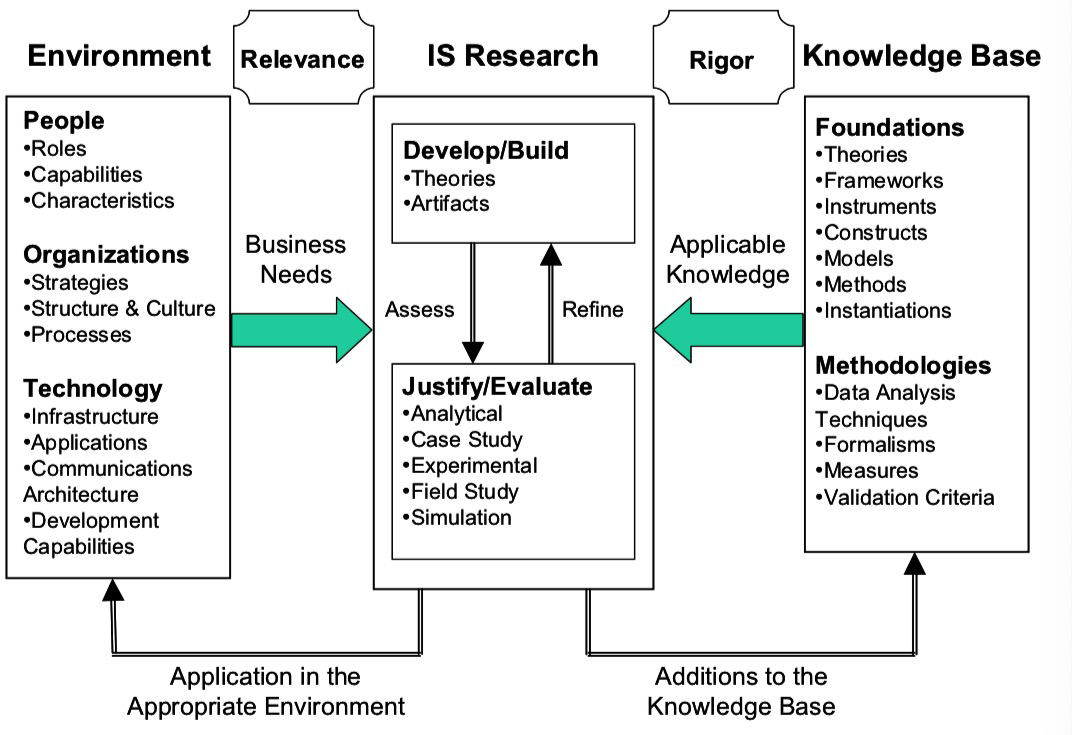
\includegraphics[width=0.75\textwidth]{isframework}
    \caption{Översikt av Information Systems Research Framework}
    \label{fig:isframework}
\end{figure}

Problemen som uppfattas av forskaren definieras i arbetsmiljön. Detta fält
består av personer, organisationer och den befintliga eller planerade teknologin
hos dem. Affärsbehoven skapas utifrån dessa tre faktorer. Organisationen
kännetecknas av strategi, struktur och kultur samt befintliga affärsprocesser.
På samma sätt formas de av rollerna, egenskaperna och kännetecknen hos
personerna i organisationen. Slutligen bidrar den nuvarande tekniska
infrastrukturen, applikationerna, kommunikationsarkitekturer och
utvecklingsmöjligheter till att definiera dem.

Personer i detta projektets arbetsmiljö utgörs således av polisstudenter liksom
lärare. Studenterna har behov av hjälpmedel i utformningen av polisrapporter på
ett rättssäkert sätt, medan lärarna å sin sida behöver få hjälp med
rättningsprocessen av dessa. Båda rollerna kännetecknas av ett mindre tekniskt
kunnande och intresse, vilket skapar behovet av ett användarvänligt system.

Organisationen som de ingår i är polisutbildningen vid Malmö universitet vars
strategi bland annat är att utbilda studenter till färdiga polisaspiranter med
kunskap att skriva polisrapporter på korrekt sätt. Den teknologi som finns till
förfogande är för tillfället läroplattformen Canvas där rapporterna lämnas in
och omdömen om dessa ges. Allt eftersom affärsbehoven definieras och genomförs är
forskningen i två faser som är integrerade med varandra. De
beteendevetenskapliga paradigmerna behandlar forskning genom utveckling och
rättfärdigande av teorierna. Samma teorier som hjälper till att förklara eller
förutsäga fenomen i förhållande till affärsbehoven.

Vår tes är att en digital språkbehandlingsapplikation som genomför automatisk
textkontroll av en rapport och återkopplar brister i denna med konstruktiv
respons kan möta de aktuella affärsbehoven för detta projekt. Ett av våra
antaganden är också att studenter genom de felmeddelanden som applikationen
återger också kan fördjupa sin förståelse för vikten av rättssäkerhet inom ramen
för polisrapporter. Konstruktionen av den applikation vi byggt, och som vi vill rättfärdiga för teorier på, beskrivs närmare i avsnittet Utveckling.

I enlighet med ramverkets rekommendation om en iterativ process i utvecklingen och utvärderandet av artefakten kommer vårt arbete att bestå av fyra stora iterationer:

\begin{enumerate}
\item Den första ska utgå från vårt initiala möte med Esbjörnsson och konkretiseras genom den kravinsamling som kommer bli resultatet av denna.
  Utifrån de önskemål och krav på artefakten som beskrivs av Esbjörnsson samt det
  officiella polismaterial som relaterar till hur rapportskrivning ska se ut
  kommer vi kunna sätta upp ramar kring omfattningen av vårt problemområde.
\item Den andra iterationen kommer bestå av den litteraturstudie vi gör för att undersöka existerande forskning som gjorts inom området, och som finns
  närmare beskrivet i \cref{relateradforskning} samt \cref{språkteknologi}.
  Utifrån denna studie kommer vi kunna justera våra forskningsmål i enlighet med det
  empiriska material vi finner. Dessa resultaten kommer också kunna leda till en insikt kring
  hur implementeringen av de olika reglerna för rapportskrivning kan ske.
\item Den tredje iterationen kommer bestå av en första instansiering av artefakten, vilket är i form av en tidig prototyp av backend och frontend, se
  \cref{fig:tidigprototyp}. Under den inledande fasen av iterationen kommer vi få tillgång till övningsmaterial bestående av uppgiftsbeskrivningar och cirka
  400 anonymiserade rapporter, där 80 redan är godkända av lärare och resten inte rättats. Vi kommer testa rapporterna mot vårt textanalysverktyg för
  att identifiera fel som inte beskrivs i den officiella polisdokumentationen,
  så som felaktiga formateringar och inkorrekta filformat, samt eventuella
  buggar i applikationen. Här kan de godkända rapporterna också hjälpa oss att
  identifiera de gränsvärden som är användbara för vår tonalitetsanalys och
  läsbarhetsanalys.
\item Resultatet av den fjärde iterationen kommer bestå av en andra och slutgiltig
  instansiering av applikationen. Denna versionen kommer vara ett resultat av de
  ändringar som görs vid utvärderingen efter användarstudien, vilka beskrivs i
  \cref{önskvärdafunktioner}, och beskrivs i sin helhet i
  \cref{applikationen}.
\end{enumerate}

Mindre iterationer kommer att förekomma i samtliga av de iterationer som beskrivs ovan. Ju
längre in i processens skede vi kommer desto mer frekventa blir dessa mindre
iterationer då vi bland annat genom instansieringarna kan identifiera fler
nödvändiga funktionaliteter. Kunskapsbasen som presenteras i ramverket består av
fundament och metodologier. Sammansatt gör dessa komponenter att forskningen kan
uppnås. Medan fundamentet skapar teorier, ramverk, instrument, konstruktioner,
modeller, metoder och instanser som används under utvecklingsfasen i
forskningsstudien skapar metodologier riktlinjer som används i berättigande- och
utvärderingsfasen. Metoden för denna process som vi ser det är tillämpningen av
språkstrategi i utformningen av polisrapporter medan instansieringen är ett
arbetssystem som visar användningen av metoden, i detta fall den applikation vi
konstruerar. Vidare finner vi våra teorier som är genomgående i fundament och
metodologier i den vetenskapliga litteratur vi tillskansat oss genom
litteraturstudien som beskrivs i \cref{litteraturstudie}. Under utvecklingen har vi
tillgång till en rad anonymiserade studentrapporter som vi kör genom
applikationen för att finna vanliga fel, detta ser vi som dataanalysteknik som
den definieras i metodologifältet.

Stabilitet för vår forskning skapas genom att tillämpa fundament med metodologi.
Då beteendevetenskap och designvetenskap tillämpas på ett företagets behov
bidrar de också samtidigt till innehållet i kunskapsbasen för vidare framtida
forskning \cite{hevner:2004}.

\subsubsection{Förkastade metoder}
Det finns andra alternativa metoder som kunde använts för att underbygga vårt
arbete, men som samtidigt av olika anledningar inte heller framstått lika
passande som Information Systems Research Framework.

En av dem är så kallad action research, en metod som kännetecknas av att den
genomförs under en pågående utbildningssession. Detta är en iterativ metod där
forskaren, i detta fallet en lärare, ständigt utforskar strategier och medvetet
analyserar resultat med avsikt att göra justeringar samtidigt som utbildningen
fortskrider \cite{clement:2004}. Då vårt arbete innefattar faktiska lärare och
sker inom kontexten av en utbildning kan action research i teorin ses som ett
passande alternativ för denna studie. Rent praktiskt anser vi dock att det vore
svårt rent logistiskt och tidsmässigt att samordna en sådan utbildningssession
som samtidigt också hade varit användbar för vår forskning.

% beskrivning av iterationsfaser

\subsection{Användartester}

Då vi eftersträvar att applikationen ska vara användarvänlig och ha hög verkningsgrad bör vi
försöka att generera mätvärden av typen UX (\textit {user experience}) som kan säkerställa
att applikationen når upp till dessa egenskaper. UX-mätvärden är baserade på ett
pålitligt mätsystem och påvisar fakta om själva användarupplevelsen. I slutändan
ska UX-mätvärden representera en del av användarupplevelsen, detta kan vara i
form av användarnas syn på effektivitet och tillfredsställelse i systemet.

UX-mätvärden kan insamlas med nästan vilken typ av utvärderingsmetod som helst,
det som avgör vilken metod som är bäst lämpad är hur många deltagare som behövs
och vilka mätvärden som ska användas. Det allra vanligaste är ett så kallat
labbtest där en mindre grupp användare deltar. I sådana test ber vanligtvis
moderatorn en deltagare att utföra ett antal uppgifter på systemet som ska
testas, därefter ställer moderatorn frågor om upplevelsen \cite{tullis:2013}.

En känd studie av Nielsen~\cite{nielsen:2000} har påvisat att endast fem användare
behövs för att generera ett optimalt användbarhetstest. Med fler deltagare
påvisar test mindre och mindre värdefulla belägg eftersom samma saker visas om
och om igen. Experter varnar dock för risken att övergeneralisera resultaten och
projicera dem på en större population utan att provstorleken är tillräcklig nog
\cite{tullis:2013}. För att minimera risken för detta ville vi vaska fram så
optimala testdeltagare som möjligt. Då de tilltänkta slutanvändarna av vår
applikation i huvudsak är polisstudenter tedde sig logiskt att vi också
utförde våra tester på dem.

Ett av de grundläggande kraven på UX-mätvärden är att de på ett direkt eller
indirekt sätt måste vara observerbara samt att de kan omvandlas till ett tal
eller räknas ihop i ett numeriskt format \cite{tullis:2013}.

Ett av de grundläggande kraven på UX-mätvärden är att de på ett direkt eller
indirekt sätt måste vara observerbara samt att de kan omvandlas till ett tal
eller räknas ihop i ett numeriskt format \cite{tullis:2013}. Av denna anledning
bestämde vi oss för att använda oss av The System Usability Scale (SUS) för att
deltagarna ska betygsätta sina erfarenheter under testet. SUS beskrivs av
Laubheimer~\cite{laubheimer:2018} som det mest välkända frågeformuläret i UX-sammanhang.

För att än mer tydliggöra vad som kan förbättras med applikationen bestämde vi
oss för att kombinera SUS med att deltagarna också ombads att besvara ett par
frågor kring systemet.

\subsection{Hot mot validitet}

Även om vårt mål är att producera så fullständiga och reproducerbara resultat
som möjligt finns det också begränsningar av slutsatserna som vi kommer kunna
dra av vår forskning.

Som det framgått i denna uppsats är vår studie nära knuten till det
digitala språkbehandlingska forskningsområdet. Sett till det empiriska material som vi
funnit under sökprocessen i vår litteraturanalys finns det en mängd betydande
studier gjorda inom detta fält. Däremot har vi märkt ett underskott på
relaterade studier av just den sortens processer, digital språkbehandling i kombination
med skriftligt utlärande, som vi själva utvecklar i detta projekt. Vi
hoppas att vår forskning ska kunna ligga till grund för liknande studier inom
dessa fält.

För att bedöma och utvärdera vår artefakt valde vi i detta arbete att använda
oss av ett användartest där fem studenter vid polisutbildningen i Malmö fick
utföra ett antal uppgifter på applikationen och därefter fylla i ett
SUS-formulär samt besvara ett antal frågor om användarupplevelsen. Vi har
ponerat risken att vi använt oss av för få subjekt vid användartestet samt
att gruppen med testanvändare även kunde ha inkluderat lärare vid utbildningen.
I hänvisning till antalet deltagare i användartestet kan vi dock motivera detta
urval genom vårt empiriska material där väl underbyggda forskningsstudier lett i
bevis att just fem användare behövs för att generera ett optimalt test. Vi menar
också att då testgruppen består av fem så specifika slutanvändare av artefakten
ger detta en god rigiditet till testet. Till detta påstår vi också att som
användartestet var utformat, inlämning samt rättning av rapporten, så hade detta
inte speglat den kontext i vilket en lärare kan tänkas använda systemet vilket
också underminerar antagandet att en lärare som testsubjekt skulle bidragit till
våra observationer av testet.

Som vi skriver i \cref{avgränsning} har vi tilldelats drygt elva veckor
för utveckling av artefakten. Det finns en risk att denna tidsram kan vara
alltför snäv och att vi till följd av detta missar att implementera kraven på
artefakten som vi samlat in genom kravinsamlingen. Som vi ser det är denna risk
återkommande vid varje större utvecklingsprojekt och således svår att hämma
annat än genom noggrannhet i arbetet och god framförhållning till projektets
slutdatum.

\section{Litteraturanalys}\label{litteraturstudie}

\subsection{Rekommendationer}

En del av vårt empiriska material förvärvades genom rekommendation, till stor del från vår
handledare Johan Holmberg. Dessa var:
\begin{itemize}
\item \textit{Language Processing with Perl and Prolog} av Pierre M. Nugues
\item \textit{Design and Creation} av Ozan Saltuk och Ismail Kosan
\item \textit{Design Science in Information Systems Research} av Hevner, Alan et.al.
\end{itemize}

I en icke-systematisk Google-sökning hittade vi Gothenburg University Computer
Linguistics som är en universitetsbaserad databas. Även om det inte gick att
göra sökningar i deras indexering gav vår systematiska genomgång av
publikationerna oss många värdefulla resultat. Här hittade vi följande artiklar:

\begin{itemize}
\item \textit{What happened? From talk to text in police interrogations} av
  Tessa C. van Charldorp
\item \textit{She had it coming?: An experimental study of text interpretation
    in a police classroom setting} av Sofia Ask
\item \textit{Huvudansatser för parsningsmetoder: Om programutvecklingens
    förutsättningar i en svensk kontext} av Kenneth Wilhelmsson
\end{itemize}

Under en icke-systematisk sökning i Libsearch, bibliotekskatalogen vid Malmö
universitet, fann vi även följande litteratur:

\begin{itemize}
\item \textit{Skrivande Polis} av Sofia Ask
\item \textit{Text och kontext : perspektiv på textanalys} av Åsa Wengelin et al.
\end{itemize}

\subsection{Sökprocess}

Då vi skulle söka igenom de databaser som fanns till vårt förfogande ansåg vi
det nödvändigt att resultaten filtreras utifrån ett antal kriterier. Dessa var
att artiklarna var skrivna på svenska eller engelska och inte publicerats
tidigare än 1990. Artiklarna var också tvungna att ha hänvisats till i minst en
artikel eller tidskrift. De nyckelord som vi ansåg vara relevanta för den här
studien var följande: \textit {digital text analysis, computational linguistics, natural
language processing}, {police} och \textit {teaching}. Vi delade sedan in sökorden och kombinationer av
dessa i sex söktermer. Att vi enbart valde sex termer berodde på att vi ansåg det vara nödvändigt att avgränsa våra resultatsträffar med hänseende till stora antal
databaser vi hade till vårt förfogande.  Söktermerna var följande:

\begin{itemize}
\item S1: ‘\textit{digital text analysis}’
\item S2: ‘\textit{computational linguistics}’
\item S3: ‘\textit{digital text analysis}’ AND ‘\textit{computational
    linguistics}’
\item S4: ‘\textit{digital text analysis}’ AND ‘\textit{computational
    linguistics}’ OR ‘\textit{natural language processing}’
\item S5: ‘\textit{digital text analysis}’ OR
  ‘\textit{computational linguistics}’ OR ‘\textit{natural language processing}’ AND ‘\textit{police}’ 
\item S6: ‘\textit{digital text analysis}’ OR
  ‘\textit{computational linguistics}’ OR ‘\textit{natural language processing}’ AND ‘\textit{teaching}’ 
\end{itemize}

Sökningarna gjordes också på svenska med sökorden översatta enligt följande: \textit
{digital textanalys (digital text analysis), datorlingvistik, datalingvistik
(computational linguistics), digital språkbehandling (natural language processing)}, {polis (police)} och
\textit {undervisning (teaching)}.

\subsection{Databaser}
Databaserna vi valde var ACM Digital Library på grund av att den är den
största databasen inom datavetenskap, IEEE Xplore Digital Library som erbjuder
4,5 miljoner dokument från publikationer inom datavetenskap och andra ämnen,
DIVA som är en databas som samlar publikationer från 47 universitet i Sverige,
Linguistics and Language Behavior Abstracts (LLBA) som samlar internationell
litteratur inom lingvistik och relaterade discipliner inom lingvistik samt
MUEP som är databasen för akademisk litteratur som skapats av lärare och
studenter vid Malmö universitet, där denna uppsats också publiceras. 

\subsection{Resultat}
Som det framgår av tabellen nedan gav våra sökningar resultat som i vissa av fallen nådde upp till tusentals träffar. I dessa fall ansåg vi det inte rimligt att gå igenom samtliga resultat på grund av den tid som en genomgång av denna magnitud hade tagit. Istället använde vi oss av en osystematisk sållning av resultaten.

I de fallen där sökningarna genererade resultat som ansågs att ta för lång tid att överskåda inledde vi med att granska rubrikerna och eventuella nyckelord av de 200 första uppsatser och journaler i den aktuella träfflistan för att på så vis finna arbeten som kunde vara relevanta för vår forskning. Efter denna gallring av resultat läste vi abstraktet av de för oss relevanta arbetena för att på så vis bestämma om de var värda att undersöka vidare. Denna sista granskning utmynnade därefter i en hämtning av arbetet från databaserna.

\begin{table}[H]
\centering
\begin{tabular}{|l|l|l|l|l|}
\hline
Databas & Sökning & Resultat & Lästa abstrakt & Hämtade artiklar \\ \hline
ACM     & S1      & 681      & 16             & 1                \\ \hline
ACM     & S2      & 18059    & 24             & 2                \\ \hline
ACM     & S3      & 61       & 6              & 4                \\ \hline
ACM     & S4      & 45       & 1              & 0                \\ \hline
ACM     & S5      & 501        & 10              & 0                \\ \hline
ACM     & S6      & 10700        & 21              & 3                \\ \hline
IEEE    & S1      & 156      & 12             & 2                \\ \hline
IEEE    & S2      & 369      & 18             & 0                \\ \hline
IEEE    & S3      & 1        & 1              & 0                \\ \hline
IEEE    & S4      & 2170     & 14             & 3                \\ \hline
IEEE    & S5      & 2435     & 20             & 0                \\ \hline
IEEE    & S6      & 33     & 33             & 1                \\ 
\hline
DiVA    & S1      & 312      & 16             & 0                \\ \hline
DiVA    & S2      & 2906     & 22             & 2                \\ \hline
DiVA    & S3      & 16       & 3              & 1                \\ \hline
DiVA    & S4      & 29       & 5              & 0                \\ \hline
DiVA    & S5      & 0        & 0              & 0                \\ \hline
DiVA    & S6      & 0        & 0              & 0                \\ \hline
MUEP    & S1      & 1245     & 31             & 1                \\ \hline
MUEP    & S2      & 380      & 15             & 1                \\ \hline
MUEP    & S3      & 209      & 11             & 0                \\ \hline
MUEP    & S4      & 531      & 12             & 0                \\ \hline
MUEP    & S5      & 175      & 8              & 1                \\ \hline
MUEP    & S6      & 225      & 12              & 0                \\ 
\hline
LLBA    & S1      & 3190     & 14             & 0                \\ \hline
LLBA    & S2      & 14580    & 16             & 3                \\ \hline
LLBA    & S3      & 492      & 10             & 1                \\ \hline
LLBA    & S4      & 10782    & 13             & 1                \\ \hline
LLBA    & S5      & 24439    & 9              & 0                \\ \hline
LLBA    & S6      & 20461    & 15              & 2                \\ \hline
\end{tabular}
\caption{Resultaten av våra söktermer i databaserna}
\label{searchtable}
\end{table}
\section{Resultat}
% motivera
\subsection{Applikationen}\label{applikationen}

Applikationen utvecklades i två olika delar. Vi utvecklade en backend som
hanterar analysen av rapporterna och en frontend som är en webbapplikation med
ett användargränssnitt som studenterna ska använda för att lämna in rapporter
och få dem analyserade. Båda delarna utvecklades iterativt, i början utvecklade
vi applikationen baserat på de önskemål som framkommit under de intervjuer vi
gjorde med vår kund på polishögskolan. Vi kunde sedan komplettera med polisens
egna dokumentation och regler för rapportskrivning samt anonymiserade rapporter
skrivna av polisstudenter som vi fått tillgång till under utvecklingens gång. I
slutet av utvecklingen hade vi skapat en färdig prototyp som vi gjorde
användartester på med studenter från polishögskolan för att kunna förbättra
webbapplikationens användargränssnitt och felmeddelandena som genereras från
backend baserat på deras feedback och våra observationer.

\begin{figure}[H]
    \centering
    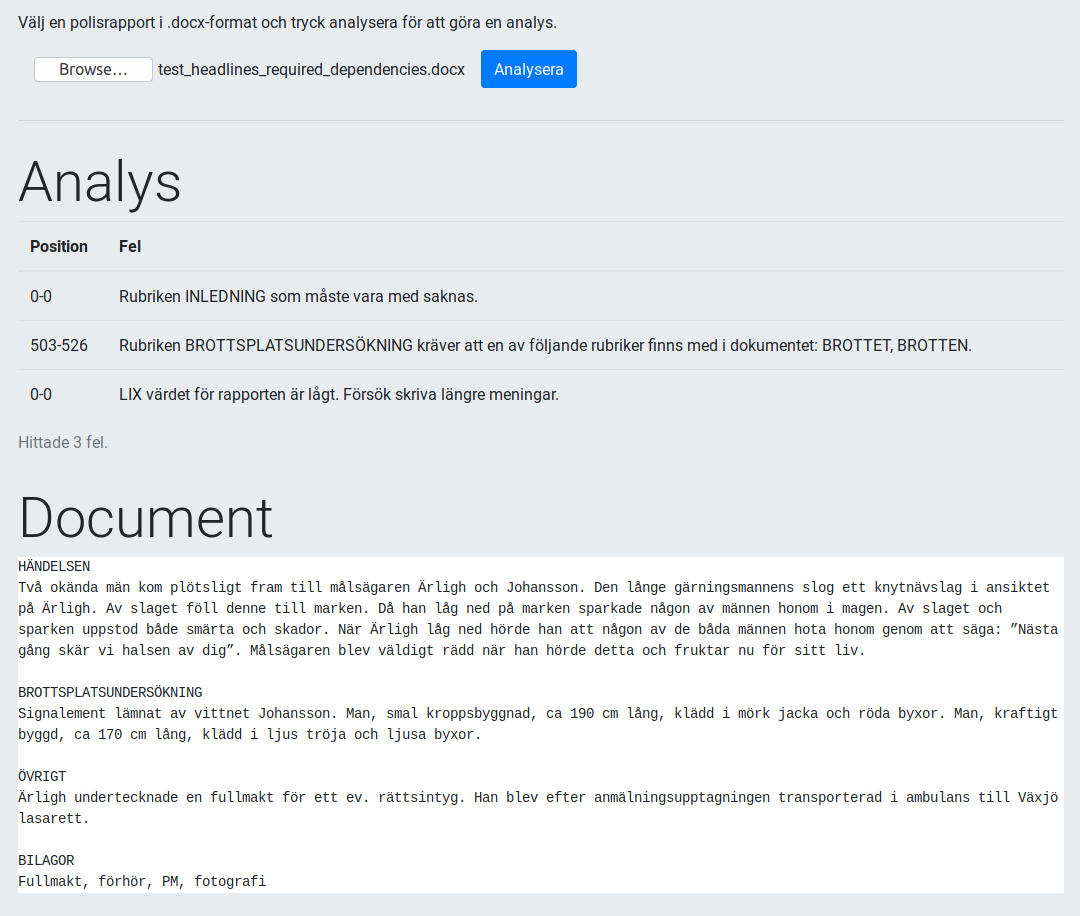
\includegraphics[width=0.75\textwidth]{tidigprototyp.png}
    \caption{Tidig prototyp av användargränssnittet i webbapplikationen}
    \label{fig:tidigprototyp}
\end{figure}

\begin{figure}[H]
    \centering
    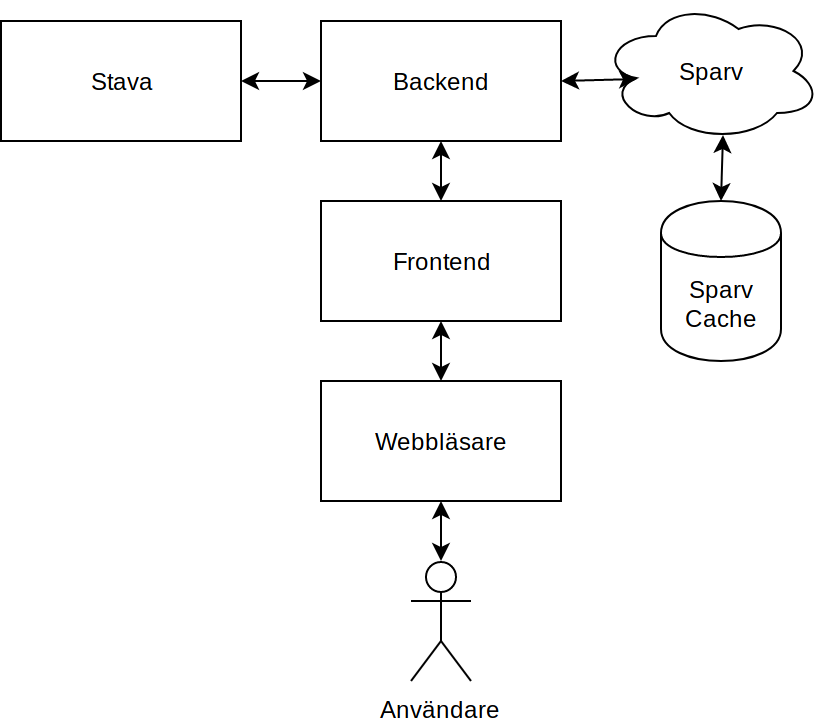
\includegraphics[width=0.75\textwidth]{architecture.png}
    \caption{Applikationens arkitektur}
    \label{fig:architecture}
\end{figure}

\subsubsection{Frontend}

Frontend utvecklades i markup-språket Hyper Text Markup Language (\textit{HTML}) för
strukturen och style sheet-språket Cascading Style Sheets (\textit{CSS}) ramverket
Bootstrap för en enhetlig design. Det är i frontend som användaren skickar in
sin rapport i docx-format och får tillbaka en analys av rapporten. Vi utvecklade
frontends användargränssnitt med integration i Canvas som mål och vi strävade
därför efter att så mycket som möjligt efterlikna Canvas grafiska gränssnitt
där man lämnar in uppgifter. Frontend är beroende av backend för att fungera
eftersom det är backend som har ansvar för att göra själva analyserna av
rapporterna. Frontend är därför bara ett gränssnitt som sköter kommunikationen
mellan backend och användaren.

\begin{figure}[H]
    \centering
    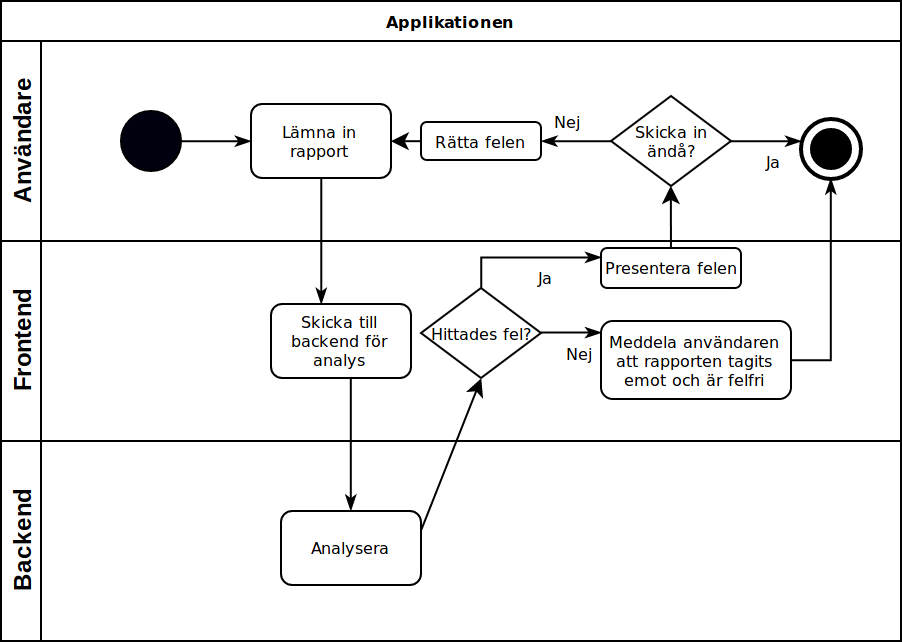
\includegraphics[width=0.95\textwidth]{overviewflow.png}
    \caption{Flödesdiagram som ger en överblick på hur man som student arbetar
      med applikationen}
    \label{fig:overviewflow}
\end{figure}

När en användare skickar in en rapport till frontend skickas den direkt vidare
till backend för analys. Ifall rapporten är felfri meddelas användaren om detta
men om rapporten innehåller fel öppnas en modal dialog för användaren där listan
på fel visas samt den analyserade rapporten i sin helhet som referens. För att
göra rättningsproccessen intuitiv och snabb kan användaren klicka på något av
felen i listan för att markera felet i referensrapporten. Felmeddelanden är
utformade så att användaren ska lära sig att undvika felen i framtiden. Detta är
viktigt eftersom de tänkta användarna är studenter som ska lära sig skriva
rapporter. Om fel hittas som användaren inte
kan eller vill korrigera ges möjligheten att skicka in rapporten utan att rätta
felen.

\begin{figure}[H]
    \centering
    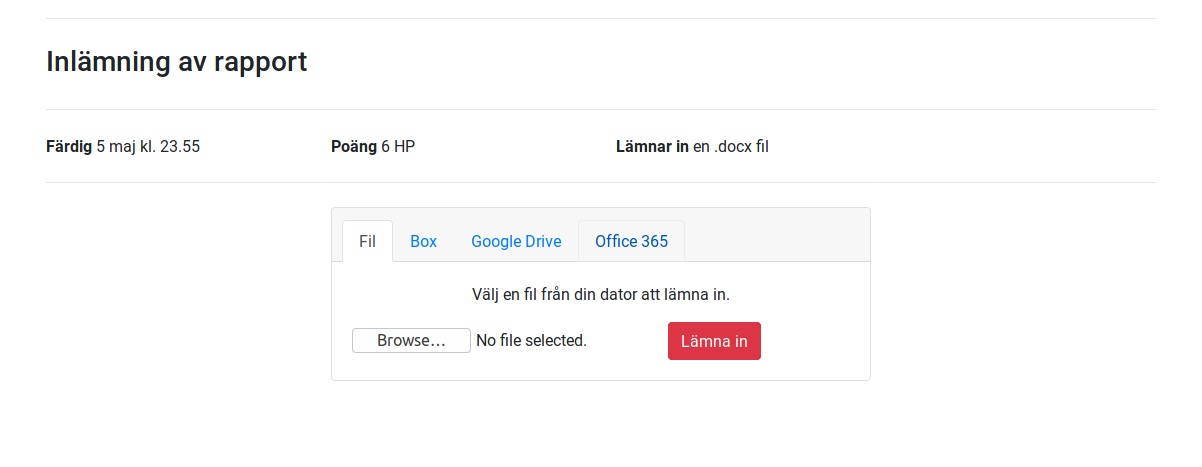
\includegraphics[width=0.74\textwidth]{frontendstart.png}
    \caption{Inlämningsdelen av frontend}
    \label{fig:frontendstart}
\end{figure}

\begin{figure}[H]
    \centering
    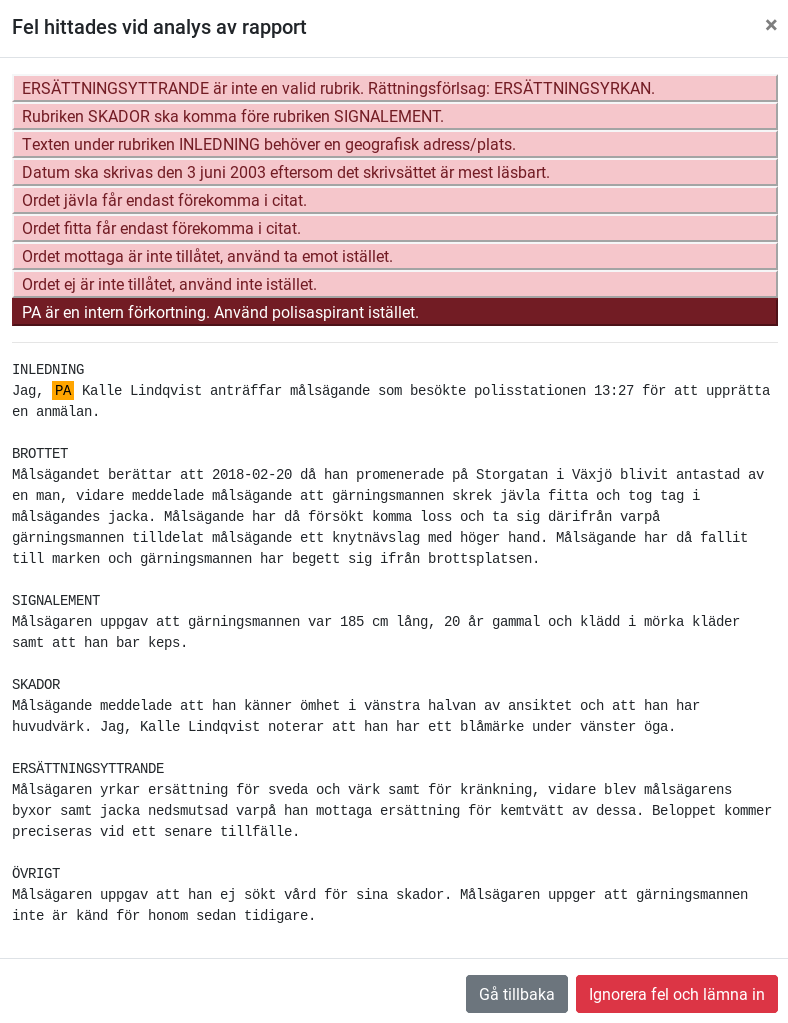
\includegraphics[width=0.75\textwidth]{frontenderrors.png}
    \caption{Frontend presenterar felen som hittades när rapporten analyserades}
    \label{fig:frontenderrors}
\end{figure}

\subsubsection{Backend}

Backend utvecklades i Python och webbramverket Flask för att ta emot och skicka
data. Backend exponerar en webbAPI som kan ta emot rapporter i docx-format
och skicka tillbaka en analys av rapporten. Vi utvecklade backend
fristående så att den fungerar utan vår frontend eftersom vi ville att det
skulle vara så lätt som möjligt att integrera i andra system som inte är
intresserade av ett användargränssnitt utan enbart APIn för att analysera
rapporter.

När en rapport tas emot i backend konverteras dess innehåll till en stor
textsträng som vår dokument-tolkare konverterar till Python-objekt. Varje
rubrik, mening, ord och identifierade namnigenkänningskategori blir objekt
vars egenskaper kommer från Sparvs textannotationer, beskrivs mer ingående i \cref{sparv}. Backend gör sedan en analys
på dessa objekt som undersöker ifall rapporten följer de regler som vi har
implementerat utifrån polisens dokumentation för rapportskrivning. De regler som
rapporten bryter mot skickas till rapportens avsändare i en lista som innehåller
felmeddelande, position och rättningsförslag för varje fel i rapporten. En
textrepresentation av rapporten skickas ihop med felmeddelanden så att eventuell
frontend får möjligheten att visa upp felpositionerna i rapporten.

\begin{figure}[H]
    \centering
    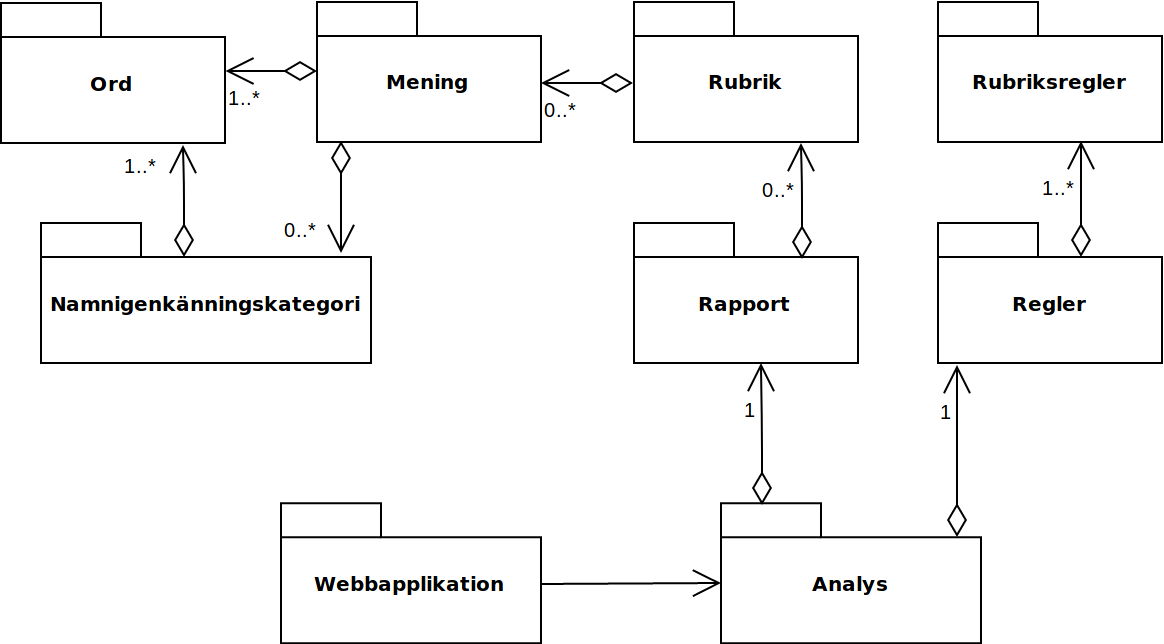
\includegraphics[width=0.85\textwidth]{backendklasser}
    \caption{Diagram som visar klasser och dess relationer i backend}
    \label{fig:erdbackend}
\end{figure}

\subsubsection{Beroenden}

Applikationen använder två externa verktyg för att göra analyser på
polisrapporterna. Anledningen till att vi här går igenom beroenden är inte
enbart för att den enskilde läsaren ska förstå hur applikationen fungerar utan
även för att göra det enklare för eventuella framtida utvecklare att
vidareutveckla applikationen. Följande rubriker beskriver vilka beroendena är
och varför vi använder dem.

\paragraph*{Sparv}\label{sparv}
Sparv \cite{sprakbanken:2019} är ett verktyg som har utvecklats av Språkbanken vid Göteborgs universitet
för att annotera texter \cite{borin:2016}. Vår applikation konverterar rapporterna till ett
specialanpassat XML-format som den sedan skickar vidare till Sparv för
annotering. De typer av annotationer vi använder från Sparv i våra analyser är:

\begin{itemize}
\item \textbf{Grundform}: Ordens grundform, ex. \textit{Bananernas} grundform är
  \textit{banan}
\item \textbf{Ordklass}: Ordens klass, ex. \textit{Kalle} är ett
  \textit{egennamn} och \textit{tjugotre} är ett \textit{räkneord}
\item \textbf{Sentiment}: Ett flyttal mellan -1 och 1. Ett positivt värde innebär att ordet har ett positivt sentiment och negativt innebär att ordet har ett negativt sentiment.
\item \textbf{Namnigenkänning}: Kategoriserar textstycken i en grupp
  fördefinierade kategorier så som geografiska platser, föremål, tidpunkter och
  många fler. Beskrivs mer ingående i \cref{namnigenkänning}
\item \textbf{Läsbarhetsindex (LIX)}: Ett mått som kan användas för att få en
  uppfattning om hur svår eller lätt en text är att läsa
\end{itemize}

\paragraph*{Stava}\label{stava}
Stava \cite{kann:2016} är ett stavningskontrollsprogram som är utvecklat av Viggo Kann och
Joachim Hollman på KTH. Anledningen till att vi valde att använda Stava för
stavningskontroll är att det är utvecklat för det svenska språket som många
stavningsprogram traditionellt sätt har svårt att hantera, Kann~\cite{kann:1997}
förklarar:

\begin{displayquote}
  Detta beror på att svenskan har många fler böjningsformer och framför allt att
  svenska ord kan vara sammansättningar som består av nästan hur många
  sammansättningsled som helst.
\end{displayquote}

Ett annat irriterande problem med rättstavningsprogram är att felstavningar av
vissa ord kan leda till att det blir ett nytt ord som är korrekt stavat men ändå
fel i sammanhanget, dessa fel upptäcks inte av rättstavningsprogram som enbart
jämför ord mot ett lexikon. Stava har löst båda dessa problemen genom att utföra
en morfologisk analys av texten och kan därmed tolka varje enskilt ords
betydelse i sammanhangen. Stava kommer med ett standardlexikon men tillåter
också att man lägger till egna lexikon vilket vi gjorde med ord som är speciella
för polisrapporter. När vi analyserar texter med Stava använder vi utöver
standardinställningarna några ytterligare regler som gör att programmet känner igen
namn, förkortningar och ger rättningsförslag, reglerna aktiveras genom att köra stava med 
argumenten \textit{-r -f -n}. En fullständig lista med alla regler kan läsas på \cite{kann:2016}. Dessa extra regler innebär att
Stava använder mycket mer datorkraft relativt mot att bara köra
standardkontrollerna. Vi tog beslutet att det var värt det eftersom
falskpositiva och missade stavfel minskar korrektheten och rättssäkerheten i
rapporterna som lämnas in med applikationen. 

\subsubsection{Textanalys av rapporter}\label{textanalysavrapporter}
% [Användarguide som bilaga]

Vi har med hjälp av Esbjörnsson, polisdokumentation och inlämnade polisrapporter identifierat, och sedan implementerat
regler som en rapport inte får bryta mot. Varje rapport som lämnas in analyseras i backend för att undersöka
ifall och i så fall hur den bryter mot någon av reglerna.
För varje fel som hittas skapas ett felmeddelande och detta meddelande beskriver vad som är fel
samt om möjligt var felet finns och rättningsförslag på hur man kan rätta det.

I \cref{rulestable} har vi skapat en lista över de regler vi har implementerat i backend.
\textit{Regel} är vad vi har valt att kalla reglen för. \textit{Lok} är ifall vi kan skicka med 
lokaliseringsinformation när en rapport bryter mot regeln och \textit{Förslag} är ifall vi kan skapa 
rättningsförslag när regeln inte följs.

\begin{table}[H]
\centering
\begin{tabular}{|l|l|l|}
\hline
Regel                                       & Lokalisering & Rättningsförslag \\ \hline
Felaktigt formatterade och saknade rubriker & Nej          & Ja               \\ \hline
Korrekt rubrik                              & Ja           & Ja               \\ \hline
Rubrikers inbördes beroenden                & Ja          & Ja                \\ \hline
Rubrikers ordning                           & Ja           & Ja               \\ \hline
Namnigenkänning                             & Ja           & Ja               \\ \hline
Läsbarhet                                   & Nej          & Ja               \\ \hline
Känsliga ord                                & Ja           & Ja               \\ \hline
Oönskade ord                                & Ja           & Ja               \\ \hline
Polisförkortningar                          & Ja           & Ja               \\ \hline
Stavning                                    & Ja           & Ja               \\ \hline
Grammatik                                   & Ja           & Ja               \\ \hline
Tonalitet                                   & Nej          & Nej              \\ \hline
\end{tabular}
\caption{Lista över regler för rapportskrivning vi har implementerat}
\label{rulestable}
\end{table}

I \cref{implementationconfigurationtable} har vi skapat en lista över vilken fil i \textit{settings/rules}~\cite{kalle:2019} konfigurationen för regeln finns och vilken metod
i \textit{src/analyser.py}~\cite{kalle:2019} där implementationen för regeln börjar.
Grammatik har ingen fil där den konfigureras utan vi kör helt på Stavas \cref{stava} inbyggda regler.

\begin{table}[H]
\centering
\begin{tabular}{|l|l|l|}
\hline
Regel                                       & Konfigurering             & Metod                                 \\ \hline
Felaktigt formatterade och saknade rubriker & rules.yaml                & test\_sanity                          \\ \hline
Korrekt rubrik                              & headlines.yaml            & test\_headlines\_predefined           \\ \hline
Rubrikers inbördes beroenden                & headlines.yaml            & test\_headlines\_dependencies         \\ \hline
Rubrikers ordning                           & headlines.yaml            & test\_headlines\_order                \\ \hline
Namnigenkänning                             & headlines.yaml rules.yaml & test\_named\_entities                 \\ \hline
Läsbarhet                                   & rules.yaml                & test\_reading\_attributes             \\ \hline
Känsliga ord                                & forbidden\_words.yaml     & test\_forbidden\_words                \\ \hline
Oönskade ord                                & rules.yaml                & test\_unwanted\_words                 \\ \hline
Polisförkortningar                          & rules.yaml                & test\_unwanted\_police\_abbreviations \\ \hline
Stavning                                    & rules.yaml                & test\_spelling                        \\ \hline
Grammatik                                   &                           & test\_spelling                        \\ \hline
Tonalitet                                   & rules.yaml                & text\_tonality                        \\ \hline
\end{tabular}
\caption{Information om konfigurering och implementation för våra regler}
\label{implementationconfigurationtable}
\end{table}

\paragraph*{Felaktigt formatterade och saknade rubriker}

Rubrikerna i en polisrapport ska vara skrivna i versaler och enbart bestå av 
alfanumeriska tecken \cite{durtva:2017}. Ifall en rapport bryter mot denna regel 
eller om rubrikerna saknas helt skapas ett felmeddelande som beskriver det godkända
formatet på rubriker.

\paragraph*{Korrekt rubrik}

En polisrapport ska vara uppdelad i olika fördefinierade rubriker
\cite{durtva:2017}. Om en rubrik som inte finns med i listan på de
fördefinerade \cite{per:2018} rubrikerna hittas skapas ett felmeddelande som beskriver felet och
ett rättningsförslag på en rubrik som kan användas istället. Rättningsförslaget
tas fram genom att jämföra Levenshteinavståndet mellan den felaktiga rubriken
med var och en av de fördefinerade rubrikerna. Den fördefinerade rubrik som har
kortast avstånd till den felaktiga rubriken blir rättningsförslaget.

Levenshteinavståndet bestäms genom att mäta det minsta antalet insättningar, borttagningar och ersättningar
som behövs göras för att två strängar ska bli lika \cite{navarro:2001}.
Det matematiska uttrycket ser ut som följer, där a och b är de strängar vi vill mäta distansen mellan:
\[\qquad\operatorname{lev}_{a,b}(i,j) = \begin{cases}
  \max(i,j) & \text{ if } \min(i,j)=0, \\
  \min \begin{cases}
          \operatorname{lev}_{a,b}(i-1,j) + 1 \\
          \operatorname{lev}_{a,b}(i,j-1) + 1 \\
          \operatorname{lev}_{a,b}(i-1,j-1) + 1_{(a_i \neq b_j)}
       \end{cases} & \text{ otherwise.}
\end{cases}\]

\paragraph*{Rubrikers inbördes beroenden}

En rubrik i en polisrapport kan vara beroende av andra rubriker, t.ex ifall
rubriken BROTTPLATSUNDERSÖKNING finns med kräver det att rubriken BROTTET också
finns i rapporten. Vi har under ett möte med Esbjörnsson~[Personlig kommunikation P Esbjörnsson 2019-01-31]
tagit fram en lista på dessa beroenden. Ifall ett beroende saknas skapas ett felmeddelande
som beskriver vilken rubrik som saknas.

\paragraph*{Rubrikers ordning}

En del av de rubriker som får användas i en polisrapport har en förutbestämd
ordning \cite{durtva:2017}, t.ex ska INLEDNING alltid vara först, BILAGOR sist
och HÄNDELSEFÖRLOPP ska alltid komma efter HÄNDELSE eller BROTT. När
analysverktyget upptäcker att rubriker är i oordning genereras felmeddelande som
meddelar användaren vilka dessa rubriker är.

\paragraph*{Namnigenkänning}\label{namnigenkänning}

Sparv använder verktyget hfst-sweNER \cite{borin:2016} för att identifiera
och annotera delar av text som faller in i förbestämde kategorier, detta kallas för Named Entity Recognition (NER). 
hfst-sweNER testar text mot tusentals olika mönster för att avgöra ifall texten 
eller delar av den faller in under någon av följande huvudkategorier \cite{kokkinakis:2014}:

\begin{itemize}
\item \textbf{Person (PRS)}: Personnamn, djurnamn etc.
\item \textbf{Location (LOC)}: Geografiska platser, gator  etc.
\item \textbf{Organization (ORG)}: Företag, politiska organisationer etc.
\item \textbf{Artifact (OBJ)}: Mat, dryck, fordon etc.
\item \textbf{Work and Art (WRK)}: Filmer, böcker etc.
\item \textbf{Event (EVN)}: Sport, Festivaler, konferenser etc.
\item \textbf{Measure/Numerical (MSR)}:  Mått, ålder etc.
\item \textbf{Temporal(TME)}: Datum, klockslag etc.
\end{itemize}

Vi har implementerat två olika typer av regler med hjälp av NER annotationer.
Den första är en regel som kommer från vårt andra möte med Esbjörnsson~[Personlig kommunikation P Esbjörnsson 2019-02-25].
Han berättade under att en del rubriker kan ha vissa egenskaper, t.ex. rubriken INLEDNING ska ha datum och plats där
anmälan togs emot. 

Den andra regeln är att datum, pengar och räkneord ska vara formaterade på
ett speciellt sätt i rapporter \cite{rfsip}, t.ex. datum ska enbart 
skrivas ``Den 21 januari 2019`` eftersom det sättet är mest läsbart.

Ifall en rapport bryter mot dessa regler skapas ett felmeddelade som beskriver
vad det är som saknas eller rätt format på det som är felformaterat.

\paragraph*{Läsbarhet}\label{läsbarhet}

Under första mötet med Esbjörnsson~[Personlig kommunikation P Esbjörnsson 2019-01-31] berättade han att en del av
rapporterna var svårlästa. Han framförde en önskan om att vårt analysverktyg
skulle kunna identifiera dessa rapporter.

Abrahamsson~\cite{abrahamsson:2011} har i sitt arbete som behandlar hur man kan göra texter
mer lättlästa tittat närmre på följande tre sätt att kvantitativt mäta läsbarhet
av text som ger ett numeriskt värde på läsbarheten:

\begin{itemize}
\item \textbf{Nominalkvot (NK)}: Mäter informationstätheten i text med följande
  formel: $$NK=\frac{Substantiv + Prepositioner + Particip} {Pronomen + Verb + Adverb}$$
  Abrahamsson~\cite{abrahamsson:2011} skriver att normalvärdet för NK ligger på 100 vilket
  kan jämföras med en tidningstext. Ett lågt NK innebär att texten är
  talspråklig och framåtdrivande och ett högt att texten är informationstät och
  tar lång tid att läsa.
\item \textbf{Ordvariationsindex (OVIX)}: Mäter hur många unika ord som finns i
  texten med formeln: $$OVIX=\frac{Unika~Ord} {Ord *100}$$
  Enligt Abrahamsson~\cite{abrahamsson:2011} är
  det svårt att tolka värdet som formlen resulterar i eftersom det helt beror på
  textens längd. En text på fem unika ord som är lättläst kommer få ett väldigt
  högt OVIX-värde medan en längre svårläst text på 20 000 ord varav 2000 är
  unika kommer få ett lägre värde.
\item \textbf{Läsbarhetsindex (LIX)}: Mäter hur avancerad en text är med
  följande formel där långa ord är ord med fler än 6 bokstäver: 
  $$LIX=\frac{Ord}{Meningar} + \frac{L\text{å}nga~ord \cdot 100}{Ord}$$
  Ett resultat under 25 är barnboksnivå, 25-30 är
  enkla texter, 30-40 är normaltext, 40-50 är sakinformation, 50-60 är facktext
  och över 60 är svåra facktexter \cite{abrahamsson:2011}.
\end{itemize}

Eftersom OVIX delvis är baserat på textens längd är det inte ett lämpligt mått då
rapporterna som lämnas in är av olika längd. Kvar är då LIX och NK. Vi bestämde
oss för att använda LIX eftersom \cite{abrahamsson:2011} skriver att det är det
vanligaste sättet i Sverige att mäta läsbarhet.

För att komma fram till värdena för en LIX-intervall som är godkänd i en rapport
undersökte vi LIX-värdet i 80 godkända polisrapporter. Medelvärdet på LIX för
dessa rapporter var 44.6 som hamnar ungefär i mitten av sakinformation-intervallen. Vi har därför valt sakinformation-intervallen som gränsen för när
vi varnar om att en text har för högt eller lågt LIX-värde.

\paragraph*{Känsliga ord}

Esbjörnsson berättade~[Personlig kommunikation P Esbjörnsson 2019-01-31] att
ett fel många studenter gör när de skriver en rapport om ett brott där en misstänkt
har använt rasistiska, homofobiska eller andra nedsättande och känsliga termer, är att 
de inte citerar dessa termer i rapporten. T.ex. \textit{Sara berättade att gärningsmannen kallade henne för jävla fitta} är fel och ska skrivas: \textit{Sara berättade att gärningsmannen kallade henne för ``jävla fitta``}. Denna regel har implementerats
genom att vi söker efter känsliga ord som inte omgärdas av citattecken och när det hittas skapas ett felmeddelande som beskriver felet.
Polisen hade ingen lista över känsliga ord utan vi har helt enkelt gjort en själva
på ord vi vet är känsliga eller nedsättande. Vi har självklart inte fått med alla 
och listan bör därför uppdateras löpande. För att slippa ha med alla möjliga böjningar
av varje känsligt ord i listan, matchar vi enbart grundform mot grundform.

\paragraph*{Oönskade ord och polisförkortningar}

Ehrenberg-Sundin~\cite{sundin:1992} har tagit fram en lista på stela ord och former som 
fortfarande förekommer i myndighetsspråk men som ska undvikas i rapporter. 
Även vissa sammansatta verb och polisförkortningar ska undvikas \cite{rfsip}.
När vårt analysverktyg identifierar någon av dessa i en rapport så skapas ett felmeddelande
som beskriver varför termen eller formen ska bytas ut och vad den kan bytas ut mot.

\paragraph*{Stavning och grammatik}

Vårt analysverktyg använder verktyget Stava för stavning och grammatik, se avsnitt \ref{stava}.
För att undvika att falskpositiva fel rapporteras till användarna rapporterar vi inte
stavfel på följande, av Sparv identifierade ordklasser: egennamn, utländska ord och förkortningar.
Dessa ordklasser identifieras ofta av traditionella rättstavningsprogram som felstavade \cite{kann:1997} trots att de är korrekta
och när vi gjorde analyser på testrapporter upptäckte vi att en del smet igenom Stava också.
När vi kombinerade Stava och ordklasserna från Sparv markerades inte ett enda ord falskpositivt i testanalyser på 40 rapporter.
När vårt analysverktyg hittar felstavade och grammatiskt inkorrekta termer skapas ett felmeddelande och rättningsförslag
ifall Stava har identifierat ett sådant.

\paragraph{Tonalitet}

Esbjörnsson [Personlig kommunikation P Esbjörnsson 2019-01-31] berättade att det är viktigt att 
rapporterna håller ett neutralt språk, även Rikspolisstyrelsen~\cite{rfsip} skriver att texten i 
rapporter ska var formellt korrekt, båda språkligt och innehållsmässigt. För att skapa numeriska värden på rapporters tonalitet följer vi Saif et al.~\cite{saif:2016} exempel för att mäta tonalitet på Twitter-meddelanden och summerar sentiment-värdet på alla ord i rapporten och summan representerar då värdet på rapportens tonalitet.

När vi skulle ta fram värden på när en rapport har fel tonalitet, alltså när den är för negativt eller för positivt skriven fick vi problem.
Vi gjorde mängdanalyser på inlämnade rapporter för att hitta lämpliga värden och upptäckte då att de negativa och positiva värden var helt beroende på
brotten som beskrevs i rapporterna. De värden vi tog fram genom att analysera 80 godkända rapporter som beskrev samma brott var bara användbart
på just den typen av brott, t.ex. kommer en rapport om att en kvinna mördats och våldtagits ha helt andra värden jämfört med en rapport om en
stulen cykel. Vi har därför valt att stänga av tonalitetsanalysen när vi analyserar rapporter. För att få analysen att fungera i framtiden
behöver vi dela upp värdena som analysverktyget varnar för beroende på vilket eller vilka brott som beskrivs. När vi skapade analysverktyget
hade vi bara tillgång till rapporter som beskrev tre olika typer av brott. Vi hoppas att vi eller någon som vidareutvecklar applikationen
kan fortsätta detta arbete, mer om detta i \cref{slutsatserochvidareforskning}.


\subsubsection{Verktyg och utvecklingsmiljö}

Både frontend och backend utvecklades i GNU Emacs 26.1 men det ska inte vara några
problem att använda andra utvecklingsmiljöer för att vidareutveckla
applikationen. Vi skrev i huvudsak applikationen i Python 3.7.3 med YAML som
konfigureringsspråk för backend samt HTML, CSS och Javascript för
användargränssnittet i frontend. För att vi skulle hålla reda på exakt version
av beroenden för applikationen använder vi Pipenv som är det officiellt
rekommenderade systemet för att hantera paket som applikationen är beroende av
och virtuella miljöer förprogram skrivna i Python. Vi använde statisk typkontroll
i all Python-kod eftersom kodbasen växte snabbt och blev uppdelad
mellan många olika filer och då går det snabbare och lättare att förstå
koden ifall metoder och variabler deklareras med typer.


\subsection{Resultat av användartester}

Användartesterna genomfördes den 9 april 2019 i ett grupprum vid Malmö
universitet. Med bistånd från Esbjörnsson lyckades vi få tag
på fem polisstudenter som deltog i vår undersökning. Eftersom vi ville undvika risken att
deltagarna skulle påverkas av varandras åsikter valde vi att genomföra testerna
med en deltagare åt gången.

De placerades vid en bärbar dator, varpå applikationen samt en polisrapport
visades. Rapporten hade framtagits av oss utifrån det urval av studentmaterial
som Esbjörnsson bifogat, och texten var preparerad med ett tiotal vanliga
fel som vi observerat utifrån dessa. Felen inkluderade bland annat oriktiga
rubriker, nedsättande termer utan citationstecken och geografisk information som
utelämnats.

Efter en kort introduktion till projektet ombads deltagarna att ladda upp den
aktuella polisrapporten de hade framför sig till applikationen och sedan
korrigera texten utifrån de felmeddelanden som visades. Datorn var kopplad till
en tv-skärm som var belägen precis bakom deltagarna, för att vi som
testledare skulle kunna observera hur testet gick.

Vi försökte ge så lite instruktioner som möjligt när deltagarna granskade
felmeddelandena och bidrog med förklaringar eller tips enbart när vi upplevde
att deltagarna blev alltför osäkra. Detta inträffade dock inte särskilt ofta.
När korrigeringarna gjorts ombads de att återigen ladda upp dokumentet. Testet
var därefter avslutat.

\subsubsection{SUS}

Deltagarna fick efter användbarhetstestet skriftligen fylla i ett SUS-formulär, vilket består av tio
numrerade frågor enligt en Likertskala i intervallen 1-5. SUS har en poängskala från 0-100, där det
slutgiltiga resultatet räknas ut i följande steg:

\begin{enumerate}
\item För varje udda numrerad fråga, ta bort 1 från det valda värdet
\item För varje jämt numrerad fråga, subtrahera det valda värdet från 5
\item Summera de nya värdena och multiplicera med 2.5.
\end{enumerate}

Vår uträkning visade att det slutgiltiga värdet blev 83,5 poäng av 101 möjliga.
Resultatet får således ses som ett gott omdöme då det är en god bit över det
genomsnittliga värdet på 68, samt över 80 poäng vilket enligt
\cite{laubheimer:2018} enbart tio procent av webbsidor hamnar i.

\subsubsection{Intervju}

Vid den korta intervjun som följde därpå fick deltagarna besvara följande fem
frågor:
\begin{itemize}
\item Var felmeddelandena tydliga eller var det något specifikt du inte förstod?
\item Är det något i processen att lämna in en rapport som är oklart?
\item Finns det något du saknar med applikationen?
\item Tyckte du något var särskilt bra med applikationen, i så fall vad?
\item Tyckte du något var dåligt med applikationen, i så fall vad?
\end{itemize}

Två deltagare var samstämmiga i åsikten att en kortare genomgång av
applikationen behövdes innan de förstod processen men att den därefter var
tydlig för dem. En deltagare sa att denne särskilt tyckte om att de specifika
felen markerades i texten när felmeddelandet klickades på, en åsikt som också
bifölls av en annan deltagare med omdömet ”det gick väldigt snabbt att se vart
felen fanns i texten”. En tredje deltagare uttryckte att applikationen ”kan vara
en jättestor hjälp till de som inte är bra på att skriva” samt att programmet
”kan vara bra på att hitta vanliga talspråksfel”. Fyra av fem deltagare
kommenterade att applikationen var tydlig som något särskilt bra.

\subsubsection{Önskad funktionalitet}\label{önskvärdafunktioner}

Två deltagare förde fram önskan att två eller flera intilliggande känsliga
termer enbart skulle resultera i ett enda felmeddelande så att det blir tydligt
att dessa ska omgärdas av samma citattecken. Vår applikation avger också
felmeddelanden om gammaldags ord och uttryck, vilket en deltagare gärna hade
sett en motivering till varför sådana ska undvikas. Samma deltagare skulle också
vilja att felmeddelande visades i en kronologisk ordning utifrån var i
dokumentet de återfanns, samt att olika färgkoder skulle kunna användas för att
gradera hur pass allvarliga de var. Personen såg även gärna att vyn automatiskt
skrollade ner till det aktuella felet efter att deltagaren klickat på felet
utöver att bara markera dess plats i texten. Två deltagare hade velat kunna
kopiera text i felmeddelandena, och då i synnerhet när det fanns
rättningsförslag, för att effektivisera korrigeringsprocessen. De ville att man
skulle kunna ändra direkt i webbgränssnittet samt att applikationen identifierar
var i rapporten den saknade tiden eller platsbeskrivningen ska föras in. I
nuläget markeras enbart rubriken där dessa saknas.

Vi valde att implementera följande funktionalitet baserat på
användarintervjuerna:

\begin{itemize}
\item \textbf{Det ska inte gå att ta bort Modalrutan av misstag}: Detta är ett
  självklart fel i användargränssnittet. Skrollknappen som man navigerar rapport
  och felmeddelanden med ligger så pass nära gränsen för modalrutan att det är
  väldigt lätt att missa och trycka precis utanför modalrutan och stänga ner den
  av misstag. Lösningen blev att låsa modalrutan och enbart stänga ner den ifall
  användaren trycker på stäng-knappen. När vi utvecklade frontend använde vi en
  stationär dator med mus vilket gör det lättare att göra precisionsklick.
\item \textbf{Felmeddelande i kronologisk ordning}: Felmeddelandenas ordning var
  baserad på ordning som analyserna kördes i backend. Detta ledde till att alla
  rubriksfel hamnade först, sedan kom alla stavfel och så vidare. Det blir mer
  intuitivt för användaren att rätta rapporten ifall felmeddelanden sorteras
  efter den ordning de dyker upp i rapporten. Lösningen blev att sortera felen
  efter den position de dyker upp i rapporten när backend skickar analysen till
  frontend.
\item \textbf{Dela inte upp intilliggande känsliga termer}: När känsliga termer
  hittades i texten så skapade vi ett felmeddelande per känslig term som
  meddelade användaren att termen bara är tillåten i citat. Ifall det kommer
  flera känsliga termer på rad i en rapport ska dessa förstås ligga i ett och
  samma citat vilket inte var uppenbart när de genererar flera felmeddelanden.
  Vi har löst detta genom att kolla ifall de känsliga termer ligger bredvid
  varandra och då genereras bara ett felmeddelande som nämner bägge termerna.
  
\item \textbf{Kopierbara felmeddelanden}: Det var vår mening att göra så att felmeddelandena inte går att kopiera eftersom användarna då kan kopiera och klistra våra rättningsförslag. Vi tror att det är viktigt att engagera användarna i rättningen av rapporten så att de förstår vad som är fel. Däremot har vi inte hittat några vetenskapliga belägg för denna tes, vilket ledde till att vi trots allt implementerade detta förslag.
\end{itemize}

De andra önskemålen implementerades inte med följande motiveringar:

\begin{itemize}
\item \textbf{Rätta rapporten i webbapplikationen}: Användaren får en lista på
  fel i webbapplikationen men måste använda sin egen ordbehandlare för att rätta
  felen. Att låta användaren rätta rapporten direkt i webbapplikationen ligger
  utan vårt scope, kravet på applikationen var att den skulle kunna analysera en
  rapport i docx-format. Det hade faktiskt varit en bra feature att ha men vi
  hade helt enkelt inte tid att implementera en ordbehandlare i
  webbapplikationen som är fullt kompatibel med Microsoft Word och LibreOffice som
  är de ordbehandlare studenterna använder när de skriver rapporter.
\item \textbf{Exakt position där platsbeskrivning och tidpunkt saknas}: Vi kan
  identifiera under vilken rubrik de saknas men inte med full säkerhet
  identifiera exakt var i texten. I de flesta rapporter som vi analyserat kan
  man inte ens som människa säga exakt var i texten de ska in eftersom de
  ofta passar in på flera ställen. Vi tror att det är bättre ifall vi överlåter
  ansvaret till användaren att bestämma hur dessa fel ska korrigeras.
\item \textbf{Motivera gammaldags ord och uttryck}: För att användargränssnittet
  ska vara effektivt kan vi inte ha långa utläggningar i felmeddelandena som
  motiverar varför polisen inte vill att man använder gammaldags ord och uttryck
  i polisrapporter. Det får räcka med att användarna får veta att de inte är
  tillåtna i rapporter, vill man sedan veta exakt motivation är det upp till
  användaren att ta reda på det själv. De tänkta användarna är dessutom
  polisstudenter och har redan fått en genomgång av reglerna som gäller vid
  rapportskrivning. När vi utvecklade applikationen skapade vi felmeddelandena
  så att de är så korta och lättförståeliga som möjligt eftersom det är svårt
  att presentera långa felmeddelanden i ett användargränssnitt på ett snyggt och
  lättläst sätt, särskilt när det är många fel som visas samtidigt.
\end{itemize}

\section{Analys}

\subsection{Applikationens effektivitet}

För att bestämma hur användbart och effektivt vårt analysverktyg är har vi genomfört två experiment.
I det första experimentet jämför vi antalet fel verktyget kan hitta mot det riktiga
antalet fel och kollar hur många fel som finns i rapporterna men som inte bryter mot
reglerna som finns definierade i analysverktyget. 

I det andra experimentet undersöker vi hur många fel analysverktyget kan hitta fel i rapporter
som har godkänts av lärare på polisutbildningen i Malmö.

I båda experimentet kollar vi även ifall analysverktyget rapporterar några fel som är
falskpositiva.

\subsubsection{Orättade rapporter}

Anledningen till att vi gjort detta experiment är för att visa att vårt verktyg är användbart som verktyg för att rätta rapporter.
Förklaring till tabellens kolumner där \textit{A} representerar de av människor hittade fel och \textit{B} är analysverktyget:

\begin{itemize}
\item \textbf{Rapport}: Identifierare för vilken rapport det är
\item \textbf{Fel(A)}: Verkligt antal fel vi identifierat som bryter mot de regler vi implementerat i vårt analysverktyg, fel som bryter mot andra regler är ej inkluderade. De som har identifierat felen i rapporterna är Per Esbjörnsson och Lotta efternamn vid Malmös polisutbildning samt vi som har skrivit applikationen, Kalle Lindqvist och Henrik Svensson. Eftersom \cref{gradedtable} visar att mänskliga rättare överlag missar ganska många fel så körde vi även analysverktyget på rapporterna för att ta fram det verkliga antalet fel.
\item \textbf{Andra fel(A)}: Hur många fel Lotta Efternamn och Per Esbjörnsson identifierat i rapporten som bryter mot regler för rapportskrivning men som vi inte har implementerat i vårt analysverktyg.
\item \textbf{Fel(B)}: Hur många fel vårt analysverktyg hittade i rapporten, falskpositiva är inte inkluderade
\item \textbf{Falskpositiva(B)}: Hur många fel av de rapporterade felen som var falskpositiva
\end{itemize}

\begin{table}[H]
\centering
\begin{tabular}{|l|l|l|l|l|}
\hline
Rapport    & Fel(A) & Andra fel(A) & Fel(B) & Falskpositiva(B) \\ \hline
1          & 10         & 0         & 10               & 1             \\ \hline
2          & 6          & 0         & 6                & 0             \\ \hline
3          & 4          & 1         & 4                & 0             \\ \hline
4          & 3          & 1         & 3                & 0             \\ \hline
5          & 15         & 7         & 15               & 0             \\ \hline
6          & 12         & 1         & 12               & 0             \\ \hline
7          & 5          & 0         & 5                & 0             \\ \hline
8          & 8          & 0         & 8                & 0             \\ \hline
9          & 6          & 1         & 6                & 1             \\ \hline
10         & 5          & 0         & 5                & 0             \\ \hline
Genomsnitt & 7,4        & 1,1       & 7,4              & 0,2           \\ \hline
\end{tabular}
\caption{Totala antalet fel och antalet fel analysverktyget hittade}
\label{ungradedtable}
\end{table}

Precis som \cref{ungradedtable} visar hittade vårt analysverktyg alla regelbrott som bryter mot de regler vi implementerat. De två falskpositiva felen som identifierades är båda två stavfel: ``torshammare'' och ``bomberkaraktär''. 
Värt att notera är att bägge falskpositiva felen hade kunnat skrivas om för att göra signalementen de beskriver klarare. De felen som identifierats men som inte bryter mot 
de regler vi har implementerat i applikationen är ungefär jämt fördelat mellan två mellanslag i rad och att punkt saknas i sista meningen under en rubrik som kräver det.
Detta visar att vår applikation är effektiv när det kommer till att identifiera de regelbrott Esbjörnsson och vi själva har identifierat som viktigast att följa när det kommer till rapportskrivning och vi uppfyller därmed
kravet att hjälpa polisstudenter att skriva rättsäkra rapporter.

\subsubsection{Rättade rapporter}

Anledningen till att vi gjorde ett test på redan rättade rapporter var för att undersöka ifall vår applikation kan hitta fel som lärare på polishögskolan missat eller släpper igenom.
Det kan också vara av intresse att ta reda på vilka typer av fel det är, ifall det bara är stavfel och grammatiska fel sker störst skada på rapportens läsbarhet men ifall
t.ex datum och tid för när anmälan är gjord saknas så invalideras hela rapporten och är därmed inte rättsäker.

Förklaring till tabellens kolumner där \textit{A} representerar de av människor hittade fel och \textit{B} är analysverktyget:

\begin{itemize}
\item \textbf{Rapport}: Identifierare för vilken rapport det är
\item \textbf{Fel}: Hur många fel vårt analysverktyg hittade i rapporten, falskpositiva är inte inkluderade
\end{itemize}

\begin{table}[H]
\centering
\begin{tabular}{|l|l|l|}
\hline
Rapport    & Fel & Falskpositiva  \\ \hline
11          & 4   & 0             \\ \hline
12          & 4   & 0             \\ \hline
13          & 2   & 0             \\ \hline
14          & 2   & 0             \\ \hline
15          & 4   & 0             \\ \hline
16          & 5   & 0             \\ \hline
17          & 5   & 0             \\ \hline
18          & 8   & 1             \\ \hline
19          & 4   & 0             \\ \hline
20          & 5   & 0             \\ \hline
Genomsnitt  & 4,3 & 0,1            \\ \hline
\end{tabular}
\caption{Fel analysverktyget hittade i rättade rapporter}
\label{gradedtable}
\end{table}

Felen som hittades är fördelade mellan följande regler, se \cref{textanalysavrapporter} för detaljerad beskrivning av
de olika reglerna:

\begin{itemize}
\item \textbf{Korrekt rubrik}:  10
\item \textbf{Rubrikers inbördes beroende}: 3
\item \textbf{Rubrikers ordning}: 6
\item \textbf{Läsbarhet}: 1
\item \textbf{Polisförkortningar}: 11
\item \textbf{Stavning}: 3
\item \textbf{Grammatik}: 8
\item \textbf{Felaktigt formatterade och saknade rubriker}: 1
\end{itemize}

Som \cref{ungradedtable} visar hittades ganska många fel i de rättade rapporterna. 
Ett rubriksfel som hittades var en rapport som använda rubriken händelse för att beskriva ett brott vilket
är helt fel eftersom rubriken händelse ska bara användas när rapporten beskriver något som hänt men som inte är ett brott.
Nästan alla rapporter innehöll rubriker som inte är med i polisens lista på godkända rubriker, kanske har studenterna
inte förstått att man inte får hitta på rubrikerna själva men då borde lärarna uppmärksamma eleverna på detta så
eleverna lär sig. Nästan hälften av alla rapporter innehöll olika interna förkortningar på polistermer.
Det är ganska allvarliga fel som hittats i rapporterna som ändå har godkänts. Hade vår applikation använts
vid inlämningen av rapporterna hade dessa fel uppmärksammats för eleverna vilket troligtvis hade resulterat
i att rapporten blivit korrekt skriven och att eleverna i framtiden hade undvikit att göra samma fel igen.


\section{Diskussion}
Hur väl har vi uppnått våra forskningsmål och frågeställningar?
\section{Slutsatser och vidare forskning}\label{slutsatserochvidareforskning}
Då kravinsamlingen som gjordes med Esbjörnsson genererade fler önskemål än
vad som bedöms görbara inom vår avgränsning tänker vi skriva lite om möjliga
infallsvinklar kring detta.
Vi skriver även om hur man kan se närmare på värden, dess gränser och ett (bättre) sätt att kolla på det.

%
% Do not change
\newpage
\addcontentsline{toc}{section}{Referenser}

\bibliographystyle{plain}
\bibliography{bibliography}

\appendix

\section{Bilaga: Användartester}

\subsection{SUS-formulär}

\begin{figure}[H]
  \centering
  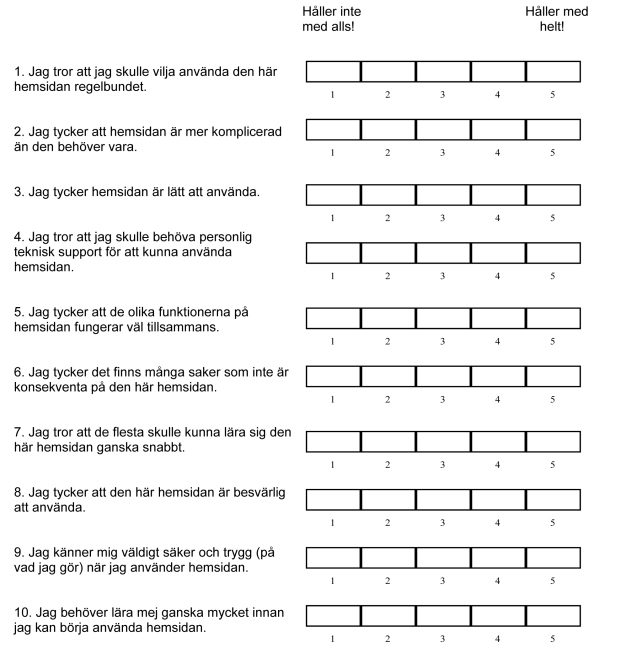
\includegraphics[width=0.75\textwidth]{bilaga/sus/form.jpg}
  \caption{SUS-formuläret vi använde}
\end{figure}

\subsection{SUS-resultat}

\begin{figure}[H]
  \centering
  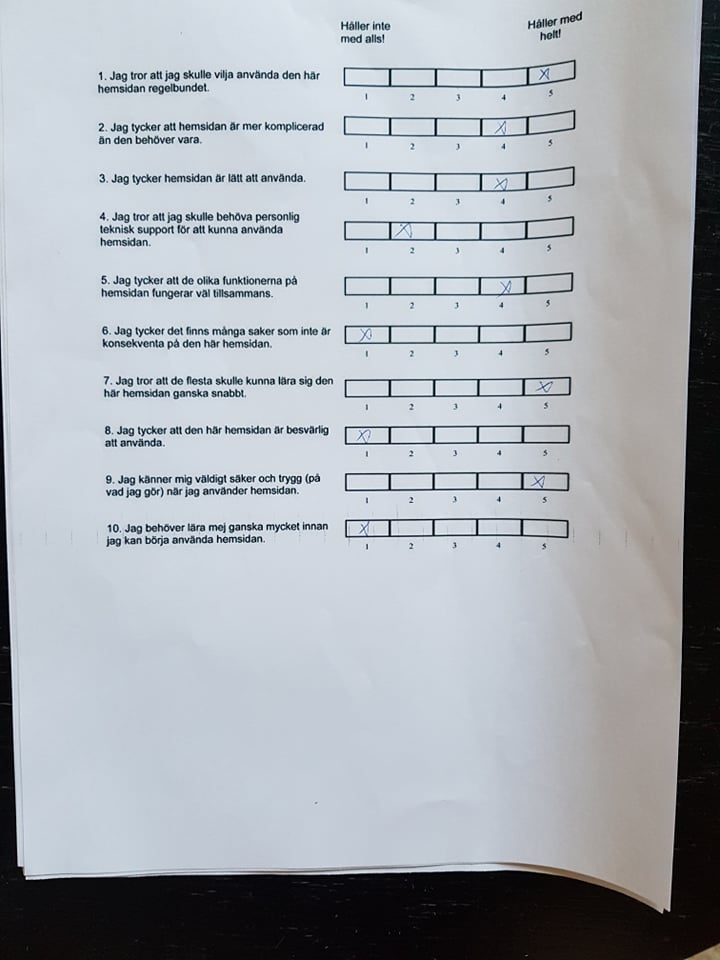
\includegraphics[width=0.75\textwidth]{bilaga/sus/ps1.jpg}
  \caption{Person 1 svar på SUS-formuläret}
\end{figure}

\begin{figure}[H]
  \centering
  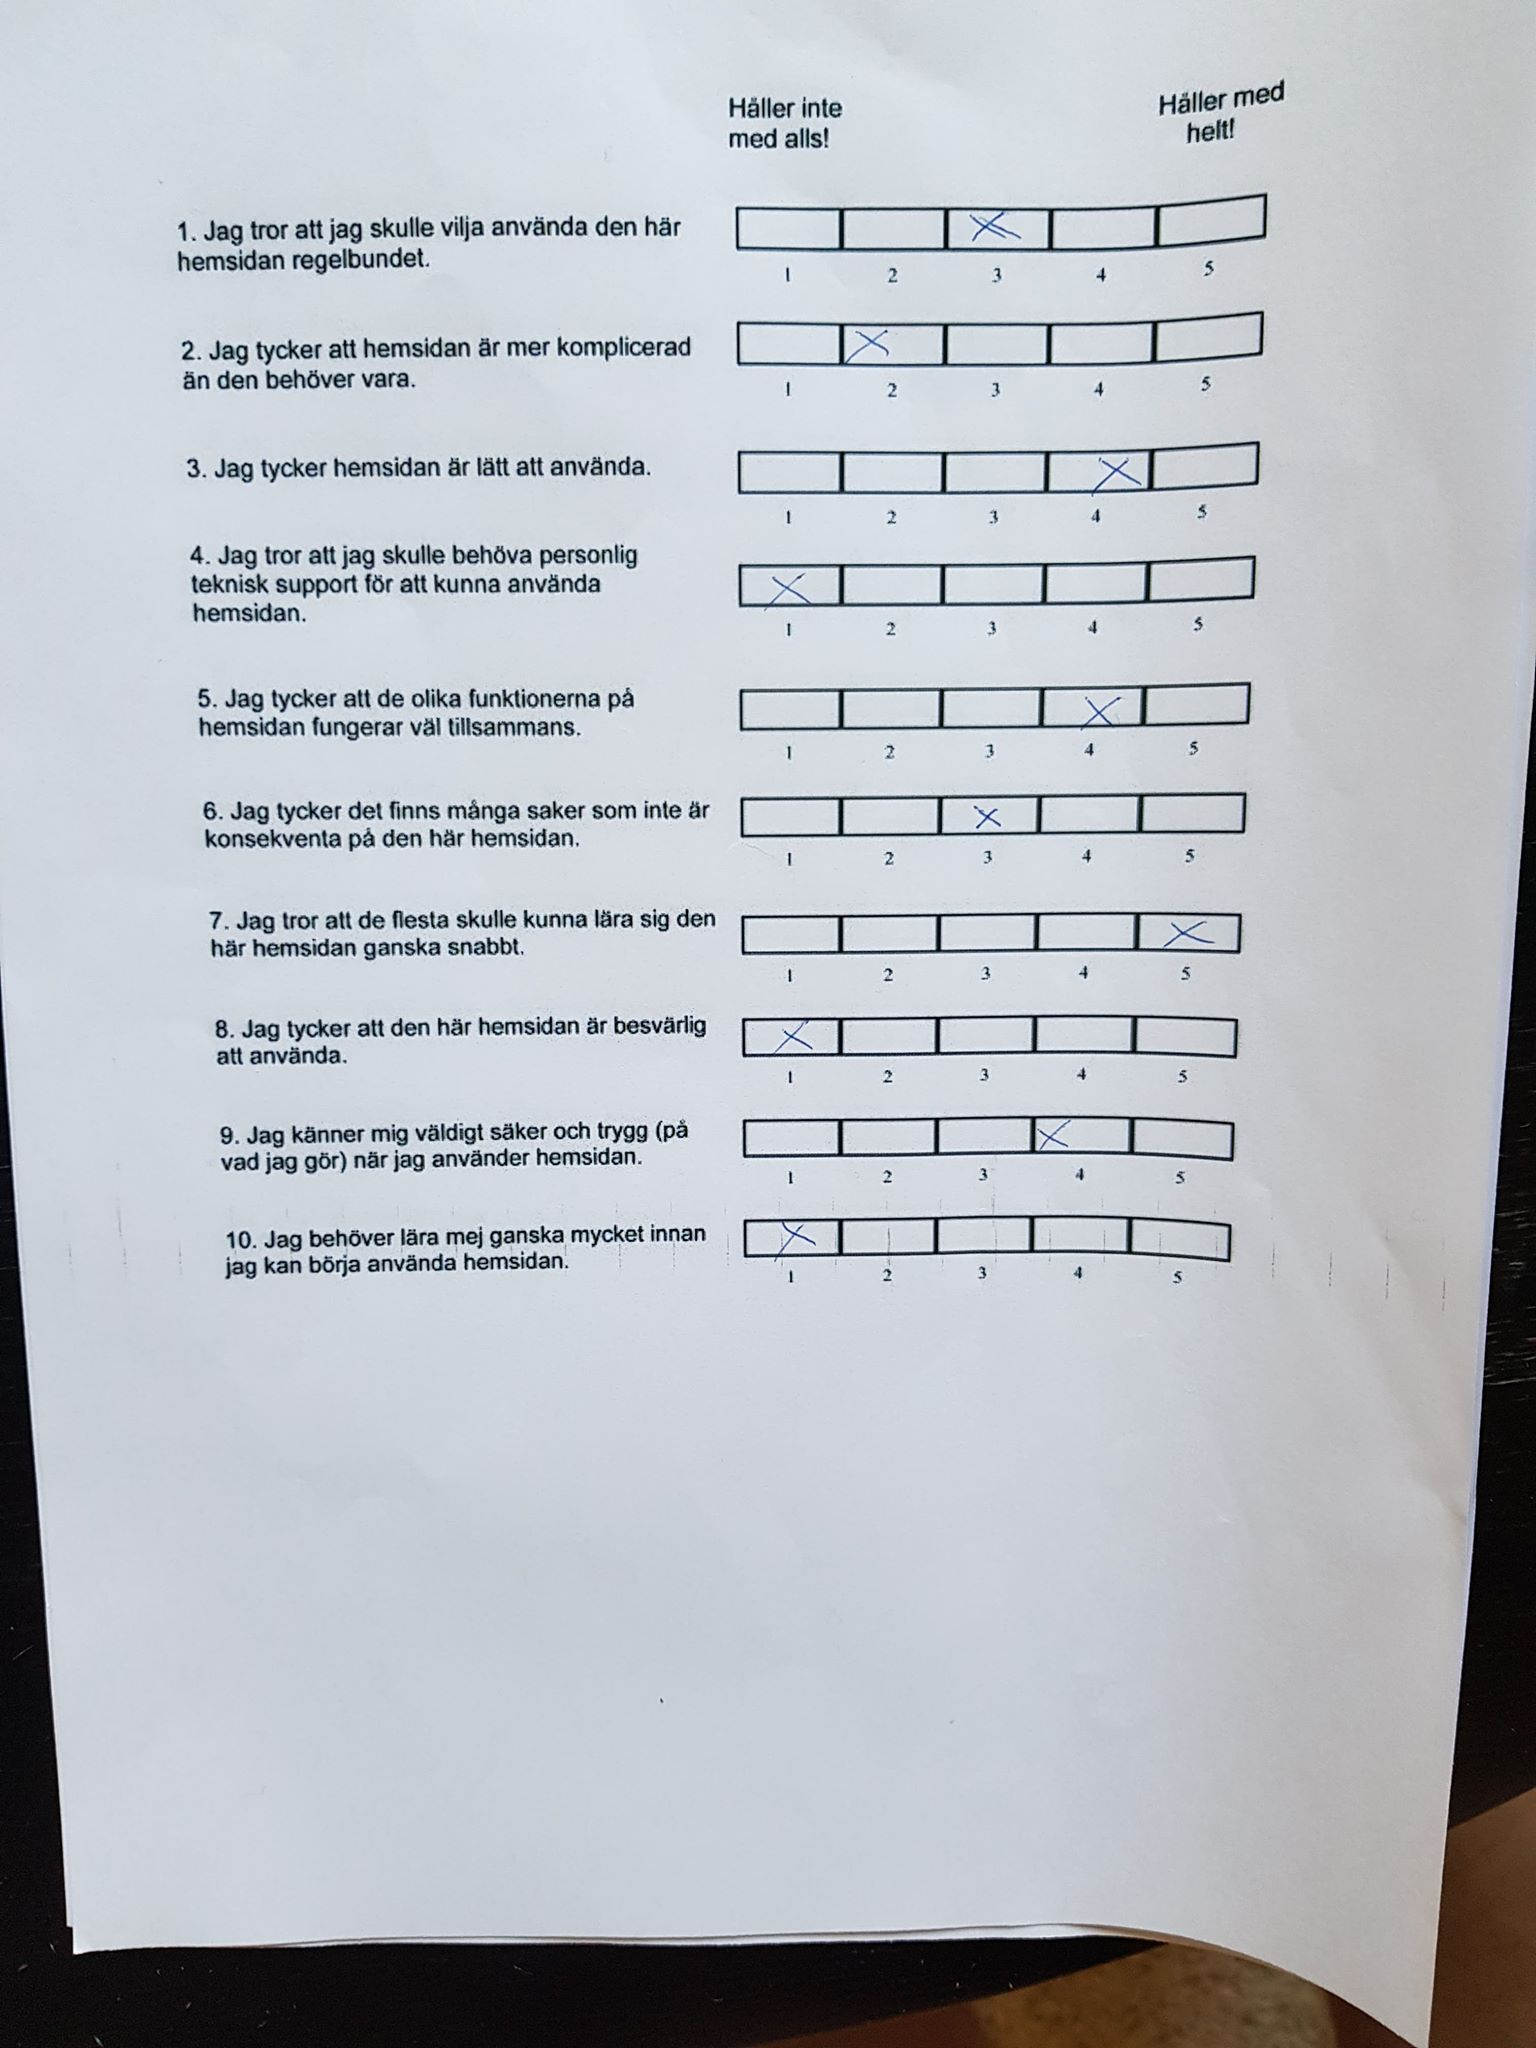
\includegraphics[width=0.75\textwidth]{bilaga/sus/ps2.jpg}
  \caption{Person 2 svar på SUS-formuläret}
\end{figure}

\begin{figure}[H]
  \centering
  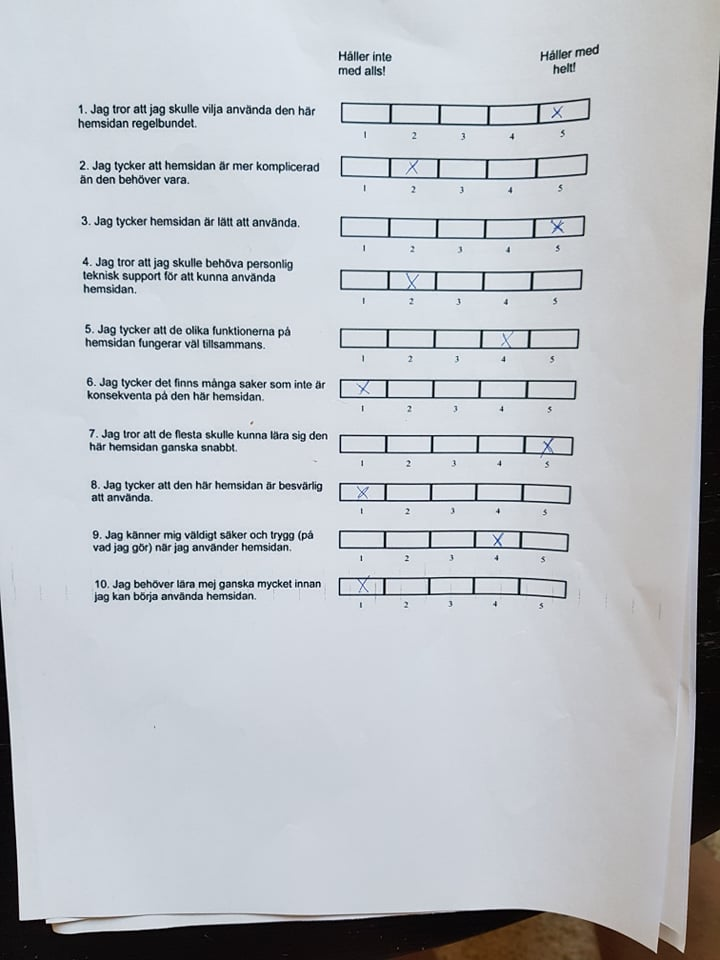
\includegraphics[width=0.75\textwidth]{bilaga/sus/ps3.jpg}
  \caption{Person 3 svar på SUS-formuläret}
\end{figure}

\begin{figure}[H]
  \centering
  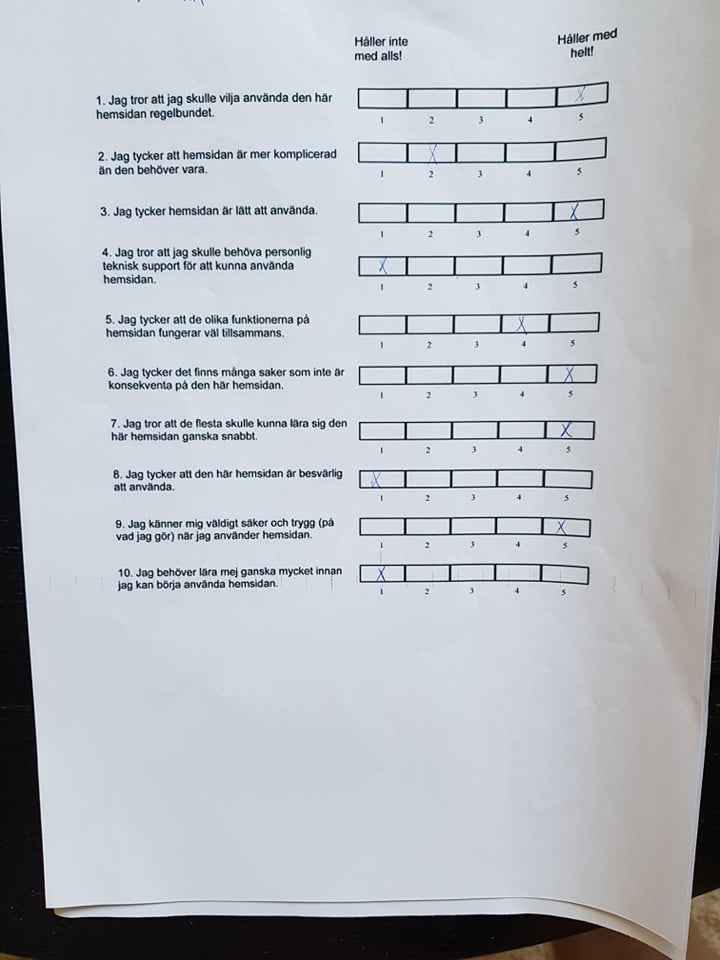
\includegraphics[width=0.75\textwidth]{bilaga/sus/ps4.jpg}
  \caption{Person 4 svar på SUS-formuläret}
\end{figure}

\begin{figure}[H]
  \centering
  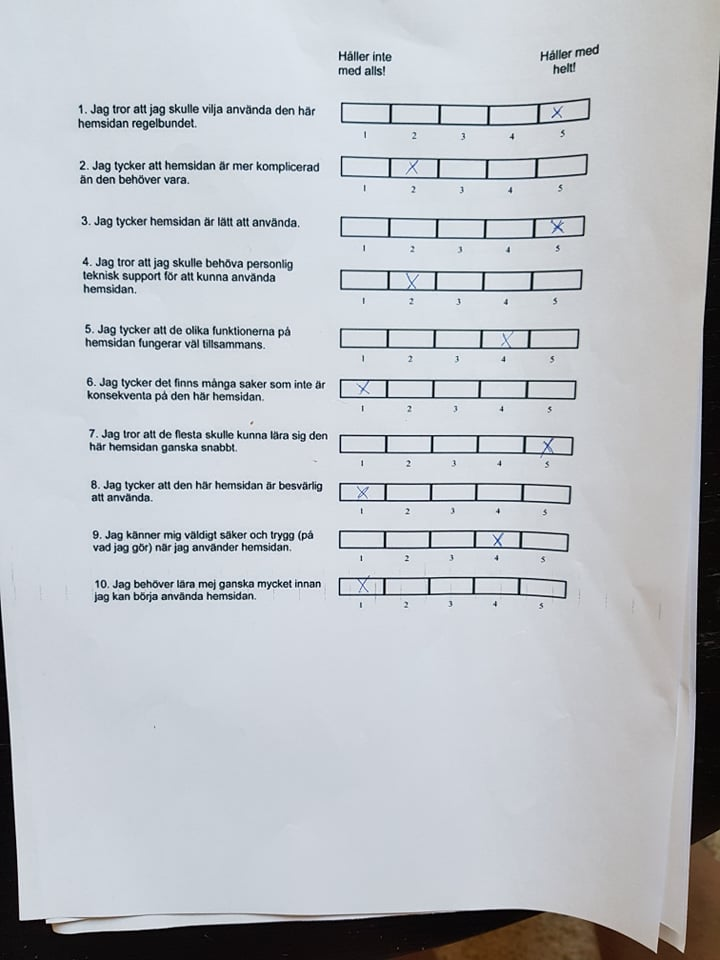
\includegraphics[width=0.75\textwidth]{bilaga/sus/ps5.jpg}
  \caption{Person 5 svar på SUS-formuläret}
\end{figure}

\subsection{Intervjusvar}

\textbf{Frågor}:
\begin{enumerate}
\item Var rättningsförslagen tydliga eller var det något specifikt du inte förstod?
\item Är det något i processen att lämna in en rapport som är oklart?
\item Finns det något du saknar med applikationen?
\item Tyckte du något var särskilt bra med applikationen, i så fall vad?
\item Tyckte du något var dåligt med applikationen, i så fall vad?
\end{enumerate}

\textbf{Person 1}:
\begin{enumerate}
\item Det var tydligt även om det var första gången. En genomgång hade dock behövts.
\item Sparningen var kanske något oklart.
\item Inget på rak arm.
\item Att man kunde se var felen fanns, att det var markerat. Gick snabbt. Att det angavs sig var rubrikerna skulle ligga.
\item Inte som han kunde se. Att allt blir rättat är viktigt, finns dock fel risk att folk skriver slarvigt första gången. Annars tummar upp.
\end{enumerate}

\textbf{Person 2}:
\begin{enumerate}
\item Att citat-varningarna kommer i två felmeddelanden.
\item Kanske om han var själv, men efter första hjälpen kan ha klara det hädanefter.
\item Nej inte direkt, förslagen är bra.
\item När man trycker så highlightas felen. Gjorde det väldigt enkelt. Kanske kan man markera geografisk plats än att enbart markera rubriken.
\item Nej.
\end{enumerate}

\textbf{Person 3}:
\begin{enumerate}
\item Nej, det står vad som ska ändras. Och vart de ska ändras.
\item Nej.
\item Inte som han kan på.
\item Citattecken-varningar.
\item Nej.
\end{enumerate}

\textbf{Person 4}:
\begin{enumerate}
\item De var tydliga, stod var det.
\item Nej, det var smidigt.
\item Hade velat ändra direkt på sidan.
\item Kan vara ett jättestort hjälp till de som inte tycker att det är roligt att skriva. Kan vara bra att hitta talspråksfel.
\item Nej.
\end{enumerate}

\textbf{Person 5}:
\begin{enumerate}
\item Man bör kunna slå ihop förbjudna ord. Motivera kanske varför man inte ska använda gammeldags ord. Man ska kunna copy-pastea.
\item Det är ganska rakt fram. Man skulle vilja rangordna felen utifrån var de är i dokumentet, eller kanske utifrån i “allvarlighetsgraden”. Kanske kan använda olikafärger för att gradera. När man klickar på ett felmeddelande så går sidan direkt till felet.
\item Nej inget direkt, känns ganska simpelt.
\item Att hitta alla fel.
\item Copy-paste-funktionen som saknas.
\end{enumerate}

\section{Bilaga: Applikationen}

\subsection{Polisrelaterade ord}



\end{document}